
%%%%%%%%%%%%%%%%%%%%%%%%%%%%%%%%%%%%%%%%%%%%%%%%%%%%%%%%%%%%%%%%%%%%%%

\chapter{Navigation Among People}
\label{chapter:navigation_among_people}

Autonomous navigation is one of the most fundamental tasks for a mobile robot. For a mobile robot with adequate actuation and sensing, collision-free navigation is considered a solved problem. There are many algorithms that achieve point-to-point autonomous navigation thanks to the advances in the motion planning community. Many of these algorithms are optimized to find the least-cost path, or the shortest path. However, when there are humans in the environment, such algorithms suddenly become inefficient or insufficient. For example, while it is acceptable for a robot to get inches close to a wall, doing so to a human is socially unacceptable and potentially dangerous. Similarly, sudden appearance of a robot can surprise or shock humans. There are many other social scenarios where the shortest path may not be optimal. 

In addition to sub-optimality, these approaches may be incomplete in the sense that they can not find a solution even though there is a feasible one. This is because shortest-path navigation algorithms treat every object in the environment as an obstacle. This assumption does not hold when intelligent agents are present in the environment. Therefore navigation should differentiate humans and obstacles for more intelligent robot behavior.

Another aspect to spatial interaction between humans and robots is the dynamics of the robot motion. For example, people may feel uncomfortable and unsafe when they are in close proximity to high-speed agents or objects. Therefore, for a robot in a human environment, while it may be acceptable to speed up in dedicated regions, its speed should be limited in places where there is a significant possibility of encountering a human.

In this Chapter, we first provide a background and present the most common approach in contemporary autonomous navigation methods in Section \ref{sec:navigation_contemporary_navigation_practices}. Second, we provide provide relevant works on navigation among people in Section \ref{sec:navigation_related_work}. Third, in Section \ref{sec:navigation_finding_goal_points_for_navigation}, we present how the goal points for navigation are determined. We then present our people-aware navigation method in Section \ref{sec:navigation_people_aware_navigation}. Lastly, we touch to the subject of introducing speed limits for all robots in a human environment in Section \ref{sec:navigation_speed_limits}.


\section{State-of-the-Art Approach in Autonomous Navigation}
\label{sec:navigation_contemporary_navigation_practices}

There are two prerequisites that enables autonomous navigation: 

\begin{enumerate}
\item The map of the environment, usually in the form of a discrete grid, that represents static objects in the environment
\item A way to localize the robot in the map using sensory information as it moves in the environment
\end{enumerate}

Robot navigation involves finding a collision-free path from a start pose $(x_{0},y_{0},\theta_0)$ to a goal pose $(x_{g},y_{g},\theta_g)$. In real-time operation, $(x_{0},y_{0}, \theta_0)$ is the robot's current pose as the robot tries to reach to the goal pose from where it currently is. $\theta_g$ is optional as the goal of the robot could be to reach the goal position regardless of its orientation. The goal position is provided from an external process, and we will touch upon how the goal positions are calculated in Section \ref{sec:navigation_finding_goal_points_for_navigation}.



\begin{figure}[ht!]
\centering
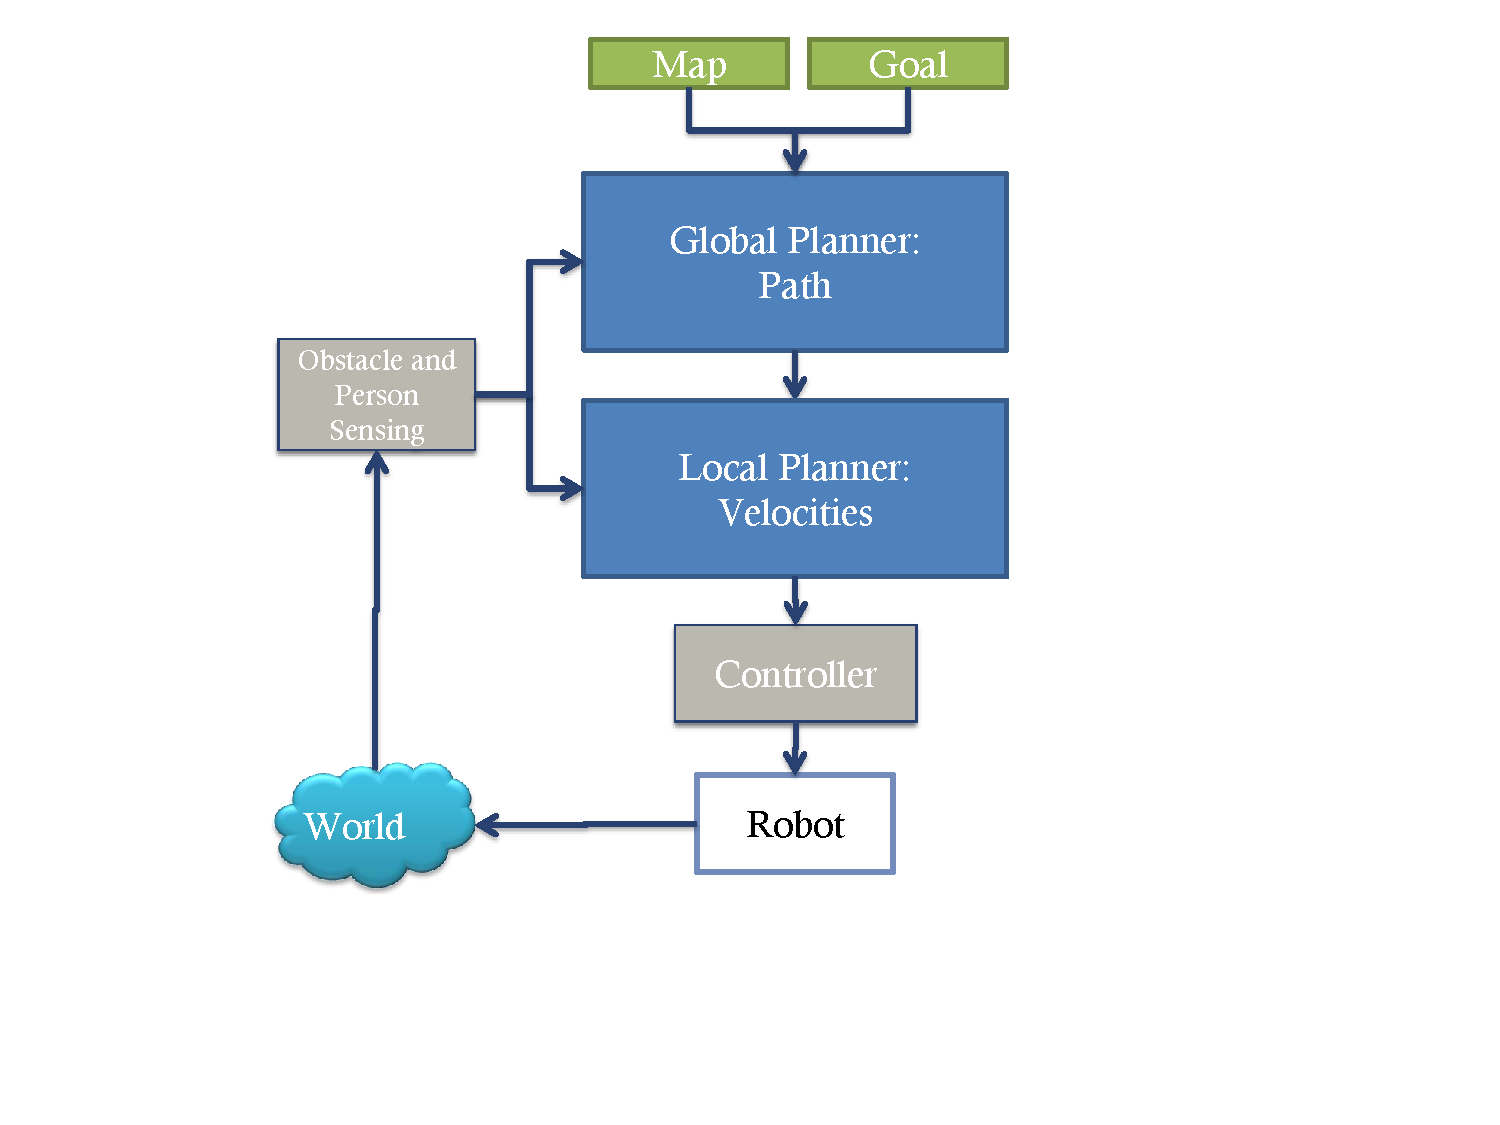
\includegraphics[width=0.5\textwidth]{pics/navigation_overview}
\caption{High-level system overview of mobile robot navigation}
\label{fig:navigation_overview}
\end{figure}

A common approach to path planning is to divide the path planning into two parts: $global$ and $local$. Global planning aims to find a path from the start position to the goal position. The global path is a set of consecutive positions that connect the start to goal position. A global path is usually found with a search algorithm executed on a graph of points. The search heuristics is dependent on specific global planners, and in most cases collision-free shorter paths are favored. The local planner is responsible to execute the global path by calculating a trajectory and sending velocity commands to motor controllers. As the robot acts in the environment, its sensors sense the new state of the robot and people, and the new iteration begins. This cycle is shown in Figure \ref{fig:navigation_overview}. 

A popular method to to implement the global and local planners is by using a $costmap$. A $costmap$ not only has the same representation as the map, however collision-free positions can have non-zero costs. A lower cost cell is more favored to be in to a higher cost cell. After the calculation of all cells, the least-cost path is found that connects the start position to the goal position.

Note that this approach assumes the robot is able to execute any path provided to it. Holonomic robots can move in any direction, however non-holonomic robots has limitations in their movements. For example, two wheel robots can not move sideways. Two common approaches to solve this problem are: to implement trajectory planners that can handle imperfect control or to embed the robot's dynamics into sampling for global and local planning.

\section{Related Work}
\label{sec:navigation_related_work}

In this section, we review the literature on robot navigation in human environments including socially acceptable navigation, learning behaviors from humans and cooperative navigation.

\subsection{Socially Acceptable Path Planning}
Socially acceptable robot navigation is considered in different applications such as free navigation~\cite{sisbot2007human}, approaching people~\cite{satake2009approach} and evacuating buildings~\cite{ohki2010collision}. Some works used the personal space concept in cost-based general path planners~\cite{sisbot2007human,kirby2009companion}. Sisbot~\cite{sisbot2007human} models the social spaces as a ellipse-shaped Gaussian, and takes into account the safety, preferences and vision fields of humans for a robot that navigates from a location to another. Kirby~\cite{kirby2009companion} presents a path planner that takes into account social conventions such as tending to one side of the hallways. A potential field based trajectory planner for dynamic human environments is presented by Svenstrup~\cite{svenstrup2010trajectory}. Rios-Martinez~\cite{rios2011understanding} presents a RRT-based planner that considers not just safety but also the disturbance of humans. In simulation, if interaction within a group of people is detected, the robot can either not disturb the interaction or join the group. This approach is implemented on a wheelchair robot~\cite{vasquez2012human}. Althaus~\cite{althaus2004navigation} presents a robot that can join a group of people and adjust to the formation reactively. The scenario where a robot encounters a human in a hallway is studied by Pacchierotti ~\cite{pacchierotti2005human}. Parameters such as the distance between the human and the robot when the robot begins to deviate from its path and lateral distance that robot should be placed when it is passing the human are found from experiments. Recent work by Lu~\cite{lu2013towards} showed that using gaze cues and social navigation makes robot-human hallway passing more efficient.

\subsection{Learning Navigation from Human Behavior}

Behaving human-like in robot navigation is usually favored in the literature~\cite{sasaki2006human}. One way to simulate human navigation behavior is to use social cost maps that capture social conventions \cite{scandolo2011anthropomorphic,luber2012socially}. Contrary to the imitation approach, \cite{bennewitz2005learning} tries to avoid predicted paths, with the goal to minimize the risk of interference. Kuderer~\cite{kuderer2013teaching} presents a tele-operated robot that computes the policy of a desired interactive navigation by learning from observations of pedestrians. Pellegrini~\cite{pellegrini2009you} trains a dynamic social behavior, that account for social interactions, using pedestrian data.

\subsection{Human Cooperation in Robot Navigation}

Robots can exploit human cooperation in certain scenarios. In populated environments, one way to move with the crowd is to follow individuals that move towards the robot's goal~\cite{stein2012robot,muller2008socially}. 

Some of the recent works in the literature claim that the robot motions should be predictable so the human observers can judge the motive and future behavior of the robot. Observational study in~\cite{lichtenthaler2013towards} claims that three features can increase the predictability of robot navigation: straight lines, stereotypical motions and usage of additional gestures. In a user study conducted by Gockley~\cite{gockley2007natural}, humans observers watched two ways of person following. People found direction-following more natural than exact path following. Kruse~\cite{kruse2012legible} observes that when paths of two humans are crossed at a right angle, they adapt their velocity rather than the path. This behavior is implemented on a robot, resulting in more predictable motions. 

Trautman~\cite{trautman2010unfreezing} introduces the 'freezing problem', where traditional path planners fail to produce a feasible solution in crowded human environments. Muller~\cite{muller2008socially} briefly mentions a 'shooing away' behavior, where the robot accelerates towards a human, hoping that he/she will get out of the way. Kruse~\cite{kruse2010exploiting} introduces an optimistic planner, which assumes that people will cooperate with robot movements. Their approach relies on assigning a non-infinite cost if a robot enters to a human's personal space, however the plan fails if humans doesn't move as expected because of the lack a local planner.

\section{Mapping and Localization}
\label{sec:mapping_localization}

Our system uses a 2-layer map:

\begin{enumerate}
\item Metric layer: Used for localization and obstacle avoidance
\item Semantic layer: Includes features such as planar landmarks, doors, navigation waypoints and objects
\end{enumerate}

In a new environment, we first run the ROS $gmapping$ Simultaneous Localization and Mapping (SLAM) package to generate the metric map. This SLAM approach is based on Rao-Blackwellized particle filter \cite{grisetti2007improved}. The front Hokuyo laser scanner at ankle level is used as the main sensor to generate the map and to localize the robot. The semantic layer is be generated by the interactive Tour Scenario (Chapter \ref{chapter:map_annotation}) and edited using the interactive Tour Scenario.

After the map is generated and saved, we localization only using this map. ROS $amcl$ package is used for localization, which implements the KLD-samping Monte Carlo particle localization approach \cite{fox1999monte}. This localization system is a local localization system, meaning it only can estimate the position of the robot given past location information. Therefore, when the robot is started, this method of localization needs a global position estimate. We offer two methods of initialization.

\begin{enumerate}
\item Manual Initialization: This is the standard method of initialization in ROS. The robot programmer provides a crude estimate to the system by clicking to a point in the map, using robot's computer.
\item Automatic Initialization using QR codes: We use a specially designed and located QR code to automatically localize the robot the first time.
\end{enumerate}

The first initialization method, in its current form, requires a robotics expert to specify the initial pose of the robot. We present our QR code based automatic initialization method here. The QR code includes links to the map and landmarks, speed limits, as well as the location of the QR pattern in the map. Therefore the robot automatically can infer its initial location upon detection of the QR code, without external intervention. System designers place QR code tags to the environment to a couple of strategic places. These places can be walls at the entrance of an indoor space, or mostly visited areas. QR codes in general contain links, text and various other data. In our application, the QR pattern includes text in XML format, which includes the link to the map and speed map files, and the position of the QR pattern in the map. Here is a sample information that a robot can read from a QR pattern:


\begin{figure}[ht!]
\centering
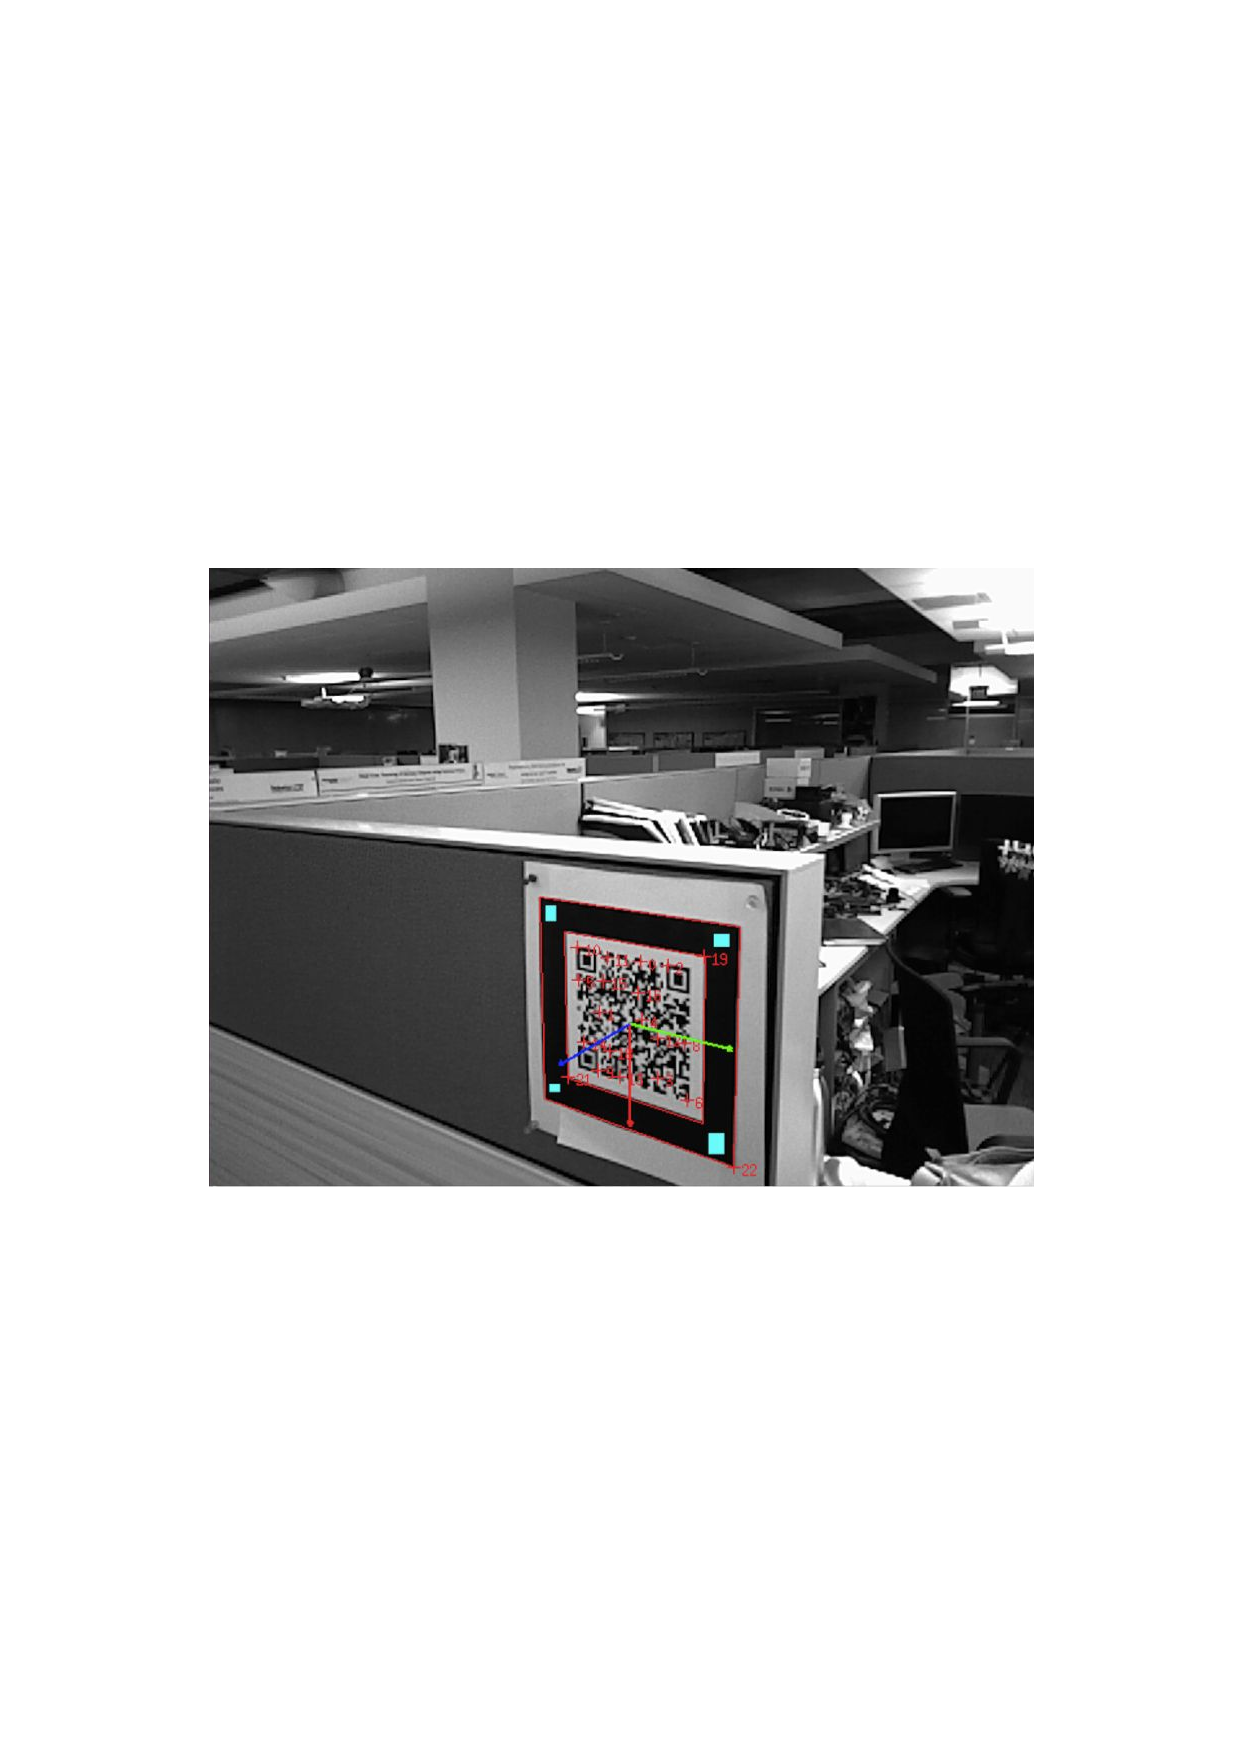
\includegraphics[width=0.6\textwidth]{pics/qrcode}
\caption{A robot can acquire map information and localize itself against the map upon detection of a specially designed QR code}
\label{fig:qr}
\end{figure}

\begin{lstlisting}
<root>
  <map>http://link1/</map>
  <speedmap>http://link2/</speedmap>
  <x>101.26</x>
  <y>98.76</y>
  <z>1.45</z>
  <q1>0.0</q1>
  <q2>0.0</q2>
  <q3>0.0</q3>
  <q4>1.0</q4>
</root>
\end{lstlisting}


The position provided in the pattern is the position and orientation (in quaternions) of the QR tag in the map frame. Using this information, a robot can acquire the knowledge of the environment automatically and locate itself in the map, where:

$^{robot}T_{cam}$ is the transformation from the robot base frame to the camera frame on the robot and is known.

$^{cam}T_{QR}$ is the pose of the QR code in the camera frame and is available upon detection of the QR code.

$^{map}T_{QR}$ is the transformation from the robot base frame to the camera frame on the robot and is read from the data embedded to the QR code.

$^{map}T_{robot}$ is the pose of the robot in the map and is unknown.\\

$^{map}T_{robot}=(^{map}T_{QR})*(^{QR}T_{robot})$

$^{QR}T_{robot}=(^{QR}T_{cam})*(^{cam}T_{robot})=(^{cam}T_{QR})^{-1} * (^{robot}T_{cam})^{-1}$

Therefore:

$^{map}T_{robot}=(^{map}T_{QR})*(^{cam}T_{QR})^{-1} * (^{robot}T_{cam})^{-1}$\\



$(x,y,\theta)$ of the robot in the map frame is required for initialization. $x$ and $y$ is readily found by looking at the displacement of the transformation. $\theta$ is found by projecting the axes to the map floor plane and . After the initial pose is provided, \textit{amcl} package handles the localization using the laser scanner readings.

We used the \textit{visp\_auto\_tracker} ROS package to extract the pose of the QR code and the content embedded in the pattern. To interpret the XML data, we used libXML++ package.


\section{Goal Points for Navigation}
\label{sec:navigation_finding_goal_points_for_navigation}

As presented in Section \ref{chapter:map_annotation}, our interactive system allows a user to annotate landmarks. After completing the $Home Tour$, the robot can navigate to or towards the labeled entities.
A user can enter a navigation destination to the robot in three distinct ways: via labeled waypoints, planar landmarks or objects.

\subsection{Labeled Waypoints:} If a waypoint is labeled and saved, the robot attaches that label to the explicit coordinates, namely position and orientation. Therefore, if the robot is instructed to navigate to a labeled waypoint, then the goal is readily the pose of the waypoint.
\subsection{Labeled Planar Landmarks:} If the label is attached to planar landmark, or a set of planar landmarks, we use the following methodology depending on the number of landmarks attached to the corresponding label:

\subsubsection{Only a single plane has the corresponding label: }
\label{sec:navigation_goal_single_label}

\begin{figure}[ht!]
\centering
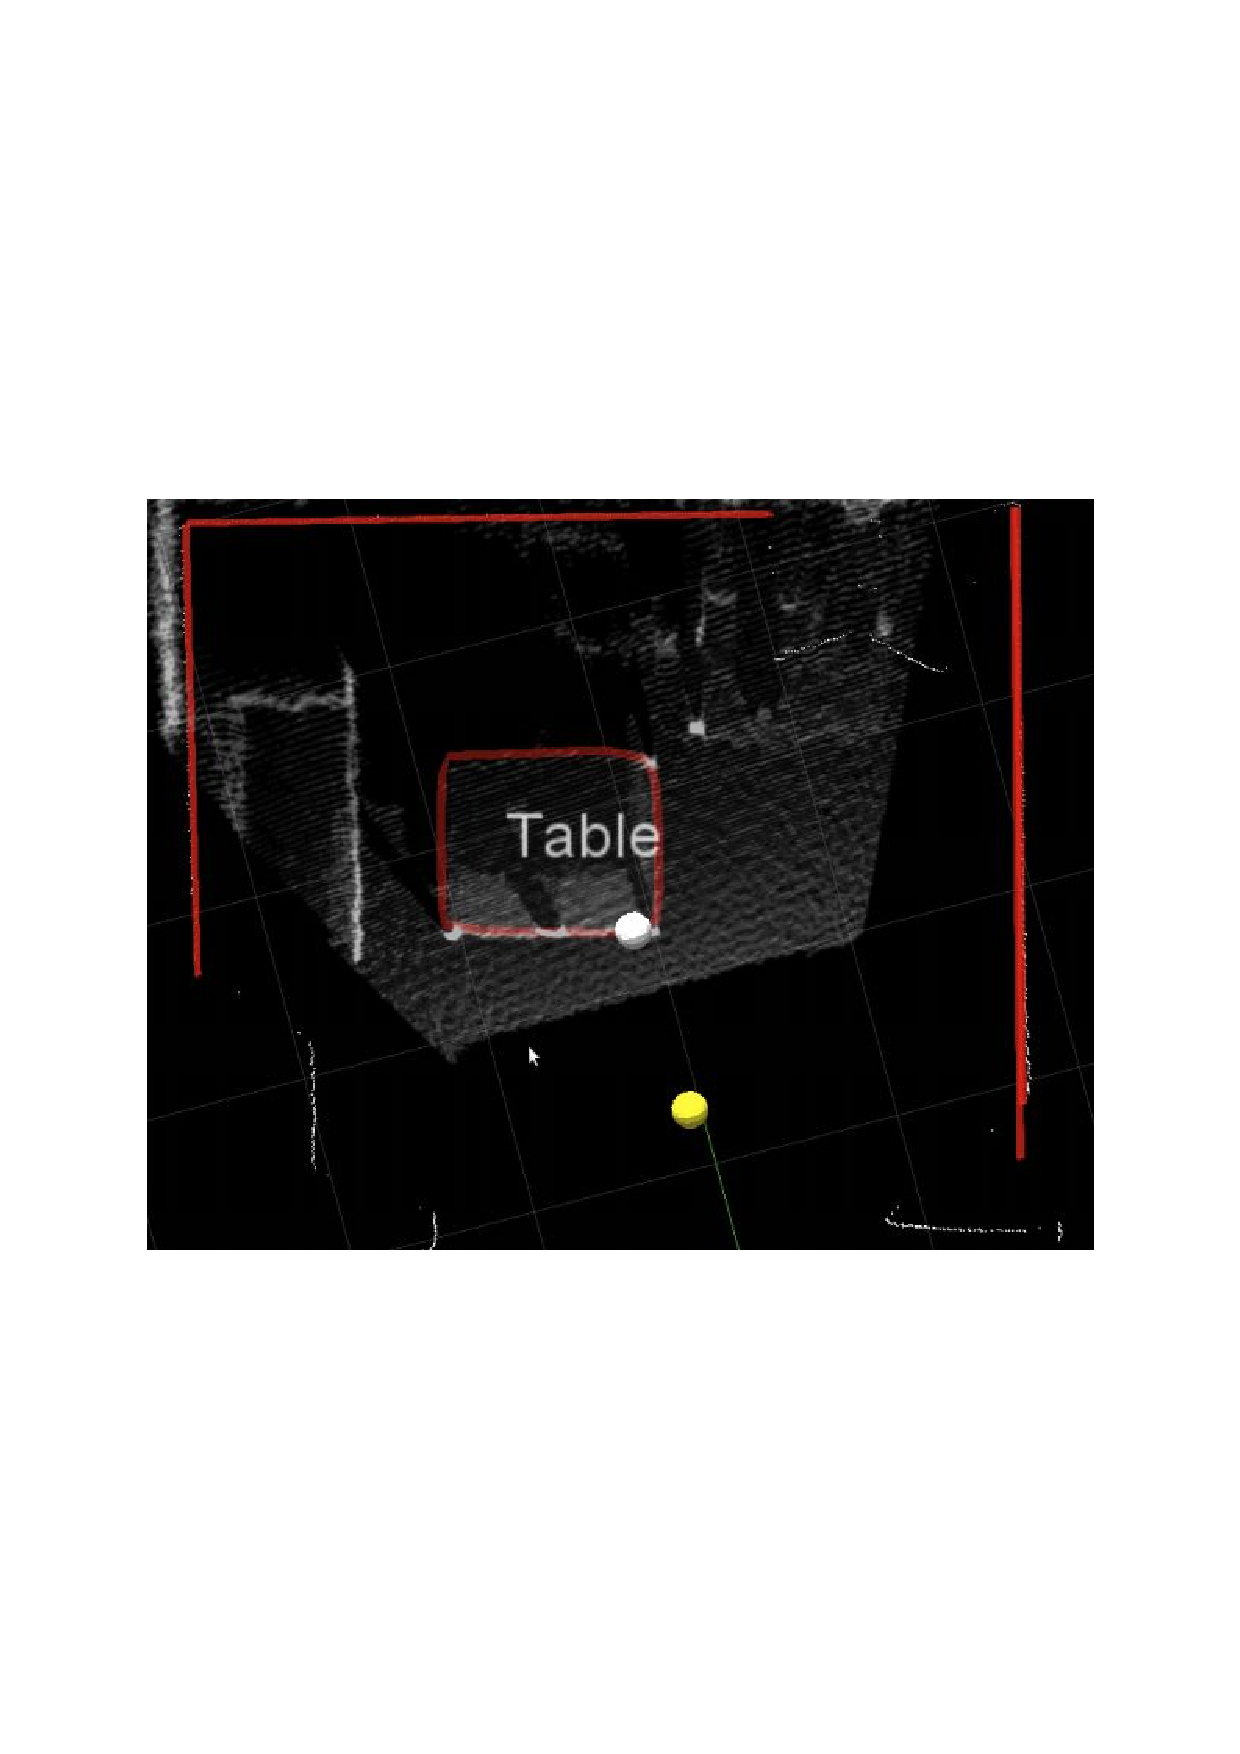
\includegraphics[width=0.6\textwidth]{pics/single_plane}
\caption{Top down point cloud view of a room. A planar landmark with label $Table$ has previously been annotated by a user. The convex hull for the planar landmark is shown in red lines. When asked to navigate to $Table$, the robot calculates a goal pose, which is shown as the yellow point.}
\label{fig:single_plane}
\end{figure}

We assume that the robot should navigate to the closest edge of the plane, so we select the closest vertex on the landmark's boundary to the robot's current position. This point is projected down to the ground plane, as our robot navigates on the floor. We calculate a line between this point and the robot's current pose, and navigate to a point on this line a meter away from the point, and facing this point. This results in the robot navigating to near the desired landmark, and facing it. This method is suitable for both horizontal planes such as tables, or vertical planes such as doors. An example for calculating a goal for a single labeled planar landmark is shown in Figure \ref{fig:single_plane}. 

where a the goal point corresponding to the singular label $Table$. 

\subsubsection{Multiple planes are attached to the same label: }

\begin{figure}[ht!]
\centering
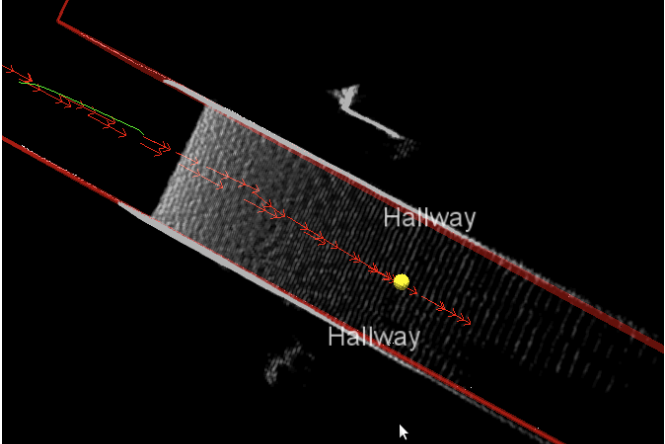
\includegraphics[width=0.65\textwidth]{pics/double_plane}
\caption{Top down point cloud view of a hallway. The user has previously annotated two planar landmarks with the same label, $Hallway$. When asked to navigate to $Hallway$, the robot calculates a goal pose, which is shown as the yellow point.}
\label{fig:double_plane}
\end{figure}

We assume that the requested label corresponds to a region of space such as a room or corridor. In this case, we project the points of all planes with this label to the ground plane, and compute the convex hull. For the purposes of navigating to this label, we simply navigate to the centroid of the hull. While navigating to a labeled region is a simple task, this labeled region could also be helpful in the context of more complex tasks, such as specifying a finite region of the map for an object search task. An example for calculating a goal for a two labeled planar landmarks is shown in Figure \ref{fig:double_plane}. 


\subsection{Labeled Objects:} As discussed in Section \ref{sec:map_objects}, we first perform planar surface detection before detecting tabletop objects. When the robot is asked to navigate to a labeled object, the planar surface that the object lies on is given as the goal landmark. The robot calculates the goal position as described in the single labeled landmark case in Section \ref{sec:navigation_goal_single_label}.

\section{People Aware Navigation}
\label{sec:navigation_people_aware_navigation}

A extensively reviewed in Section \ref{sec:navigation_related_work}, people-aware navigation algorithms aim to generate human-friendly paths that consider the safety and comfort of people. A common assumption for point-to-point people aware navigation is that humans are independent agents and that robot's motions have no effect on people's motions. However, humans navigate by constantly anticipating other people's reactions. Similarly, mere presence of a robot in motion is likely to influence how nearby humans would move. 

Robots can potentially use this implicit cooperation between moving embodied agents. For example, consider a robot that is outside a room and given a goal pose in the room. There is a person standing at the door and blocking the path. Such an example is illustrated in Figure \ref{fig:room}. Standard path planners, as well as planners that consider dynamic objects fail to produce a solution to this problem. The role of physical embodiment in human-robot interaction is significant~\cite{wainer2006role}, however it is commonly ignored in robot navigation. A people-aware planner should anticipate that the human may give way to the robot if it expresses its intent to go inside the room. Extending this idea, by using anticipation a robot can reduce its time of travel and behave more human-like in general cases.

\begin{figure}[t!]
\centering
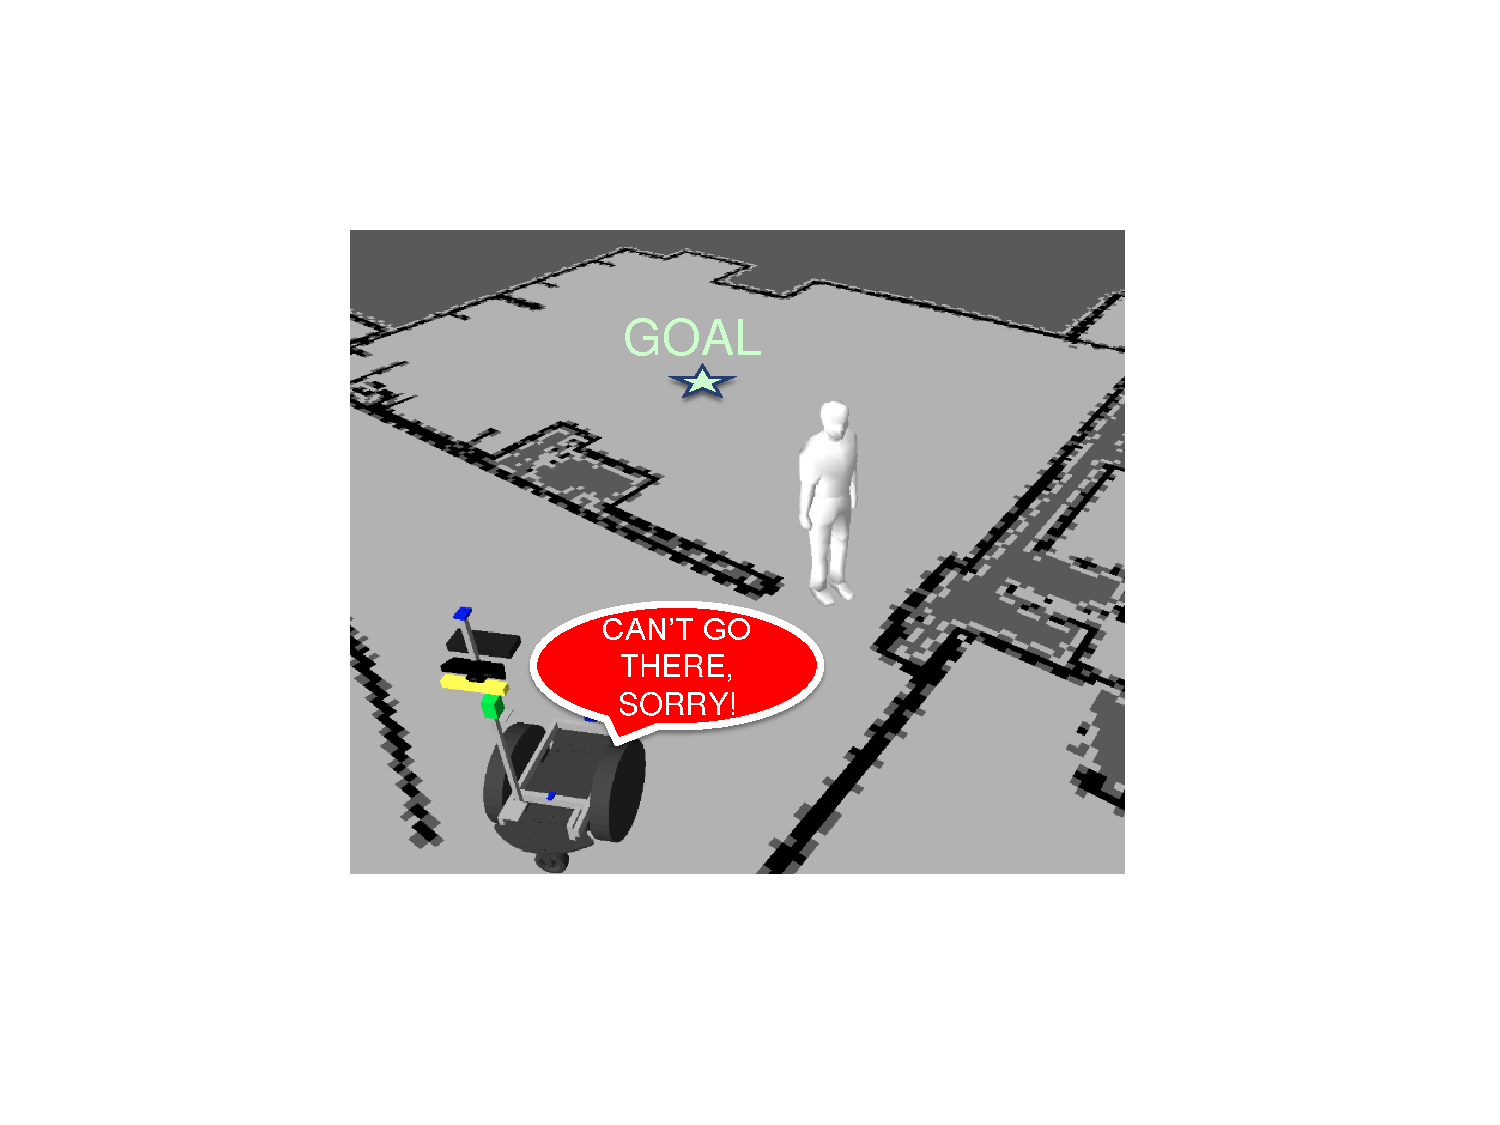
\includegraphics[width=0.5\textwidth]{pics/room_crop}
\caption{Standard path planners fail to produce a solution to the 'room problem'. Our people-aware planner anticipates that the human can give way to the robot if it approaches towards its goal.}
\label{fig:room}
\end{figure}

In this section, we propose a people-aware navigation planner that considers reactions of humans to robot motion. Our planner first first finds the least-cost map in the costmap that considers safety and disturbance of people. The costmap definition is discussed in Section \ref{sec:navigation_global_planner}. Then the path is refined by simulating people's reaction to robot's motion using Social Forces Model~\cite{helbing1995social}. The path refinement will be discussed in Section \ref{sec:navigation_path_refinement}. In dynamic simulation, robots and humans repulse each other, and additional forces helps to stay away from obstacles and conserve formation in groups. Paths are re-planned when the world state changes or humans does not move as anticipated. In Section \ref{sec:navigation_local_planner}, we discuss our local planner. We then discuss the implementation of the system in Section \ref{sec:navigation_results}, demonstrate two example scenarios in simulation in Section \ref{sec:navigation_results_simulation} and two on the real system in Section \ref{sec:navigation_results_real_robot}.


\subsection{Global Planner}
\label{sec:navigation_global_planner}

The global planner takes the start and goal positions and a 2D grid map as input and aims to find a set of waypoints that connects the start and goal cells. The output path has the minimum cost with regards to a cost function with 3 parameters: path length, safety and disturbance. We use A* search with Euclidean heuristics on a 8-connected grid map to find the minimum cost path. The configuration space obstacles are found by inflating the map obstacles for as much as the radius of the robot with the assumption that the robot is circular.

\textbf{Path length cost:}  Each action $a$ of the robot (moving to one of the 8 adjacent cells) has a non-negative action cost $Cost_{a}(x_{i},y_{i},a)$. If the destination cell is occupied by a configuration space obstacle, then the action cost is infinite. Otherwise, it is the distance in meters. The action cost is thus defined as:
\begin{align}
Cost_{a}(x_{i},y_{i},a)=\left\{ \begin{array}{cl}
u & \textrm{if $a$ = N, E, S, W}\\
u\sqrt{2} & \textrm{if $a$ = NW, NE, SW, SE}\\
\infty & \textrm{if  $Cell(x_{i+1}, y_{i+1})$ in obstacle} \end{array}\right.
\end{align}
where N,NW,.. are the grid cell expansion directions and $u$ is the grid cell size. The resulting path length cost of a path $P$ is then the sum of all action costs: 
\begin{align}
Cost_{path}(P) = \sum\limits_{a \in P} Cost_{a}(x_{i},y_{i},a)
\end{align}

\textbf{Safety cost:} The notion of safety is the absolute need of any human-robot interaction scenario. This cost is a human centered 2D Gaussian form of cost distribution and aims to keep a distance between the robot and the humans in the environment. While some approaches used un-isotropic cost functions to account for human orientation, we use a isotropic Gaussian for its simplicity. Each cell coordinate around a human contains a cost inversely proportional to the distance. Since the safety loses its importance when the robot is sufficiently far away from the human, safety cost becomes zero after a threshold distance. If there are multiple people in an environment, the safety cost of a cell takes its value from the closest human.
\begin{align}
Cost_{safety}(x,y)=\left\{ \begin{array}{cl}
u\max_{h\in H}(\mathcal{N}(\mu_h,\sum)) & \textrm{if $d<d_{max}$}\\
0 & \textrm{if $d\geq d_{max}$}\\
\end{array}\right.
\end{align}

where d is the distance to the closest human, H is all humans, $\mu_h = (|x - h.x|,|y - h.y|)$ and $\sum = 0.5I_2$ is a fixed covariance matrix. The multiplication by the grid cell size compensates for the grid map resolution. Otherwise, for example, if a very fine map was used, safety cost would dominate the path length and disturbance costs, which are independent of the map resolution.
 
\textbf{Disturbance cost:} This cost is aimed to represent the cases where the robot potentially disturbs the interaction of a group of humans. For example, if two people are facing each other and talking, then the robot should not cross between them.  We model this with a disturbance cost that is introduced if a path crosses between two people. We do not detect if there actually is conversation between the people, but estimate the disturbance cost using body poses of agents. This cost increases if body orientations of two people are facing each other and is inversely proportional on the distance between the two humans.

For each step taken in the grid, we check if the line segment from the current position to the  projected position intersects a line segment between all pairs of humans. To illustrate, let's assume the robot crosses the line between human A and human B in Figure~\ref{fig:disturbance}. 

The disturbance cost is calculated as:
\begin{align} 
\begin{split} 
Cost_{dist}(x,y,a)&=\max(0, f(d).(\vec{AA'}.\vec{AB}+\vec{BB'}.\vec{BA})) \\
f(d)&=\frac{1}{d}-\frac{1}{d_{max}}
\end{split} 
\end{align}

where all the vectors are normalized and $d_{max}$ is the maximum distance between the humans that returns a disturbance cost. Figure~\ref{fig:disturbance_ex} illustrates several examples of disturbance costs with $d_{max}=3$ meters.

\begin{figure}[ht!]
\centering
%
        \subfigure[]{%
            \label{fig:disturbance}
            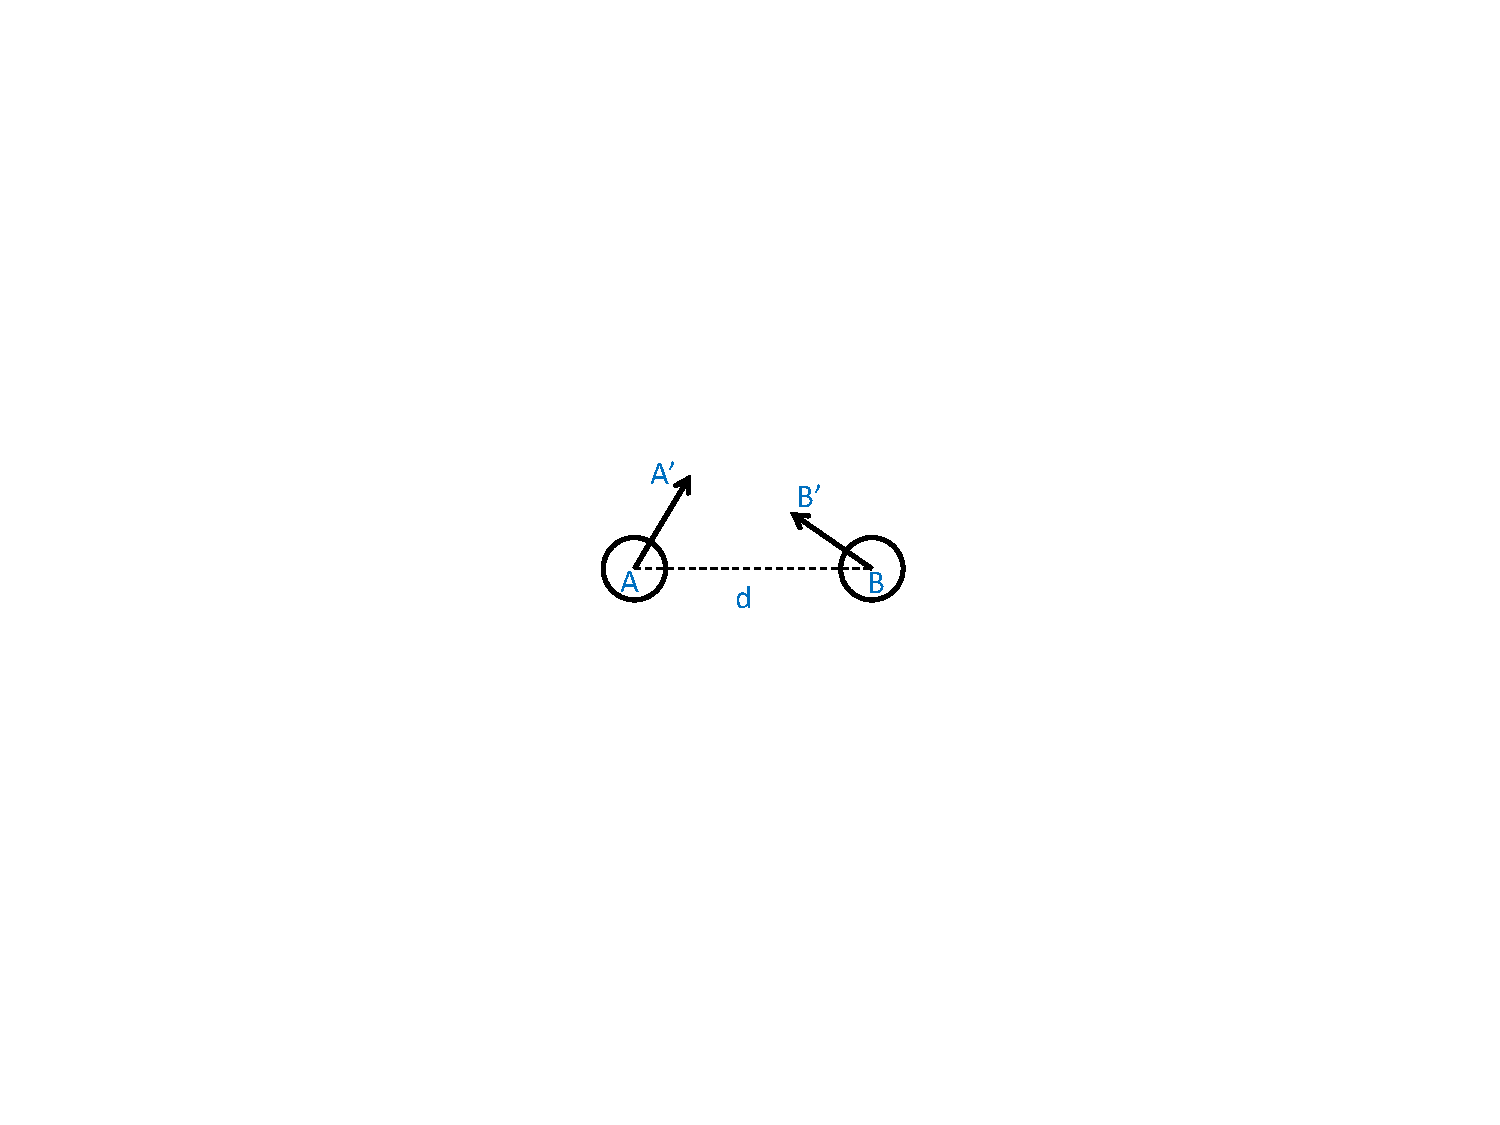
\includegraphics[width=0.32\textwidth]{pics/disturbance_crop}
        }%
        \subfigure[]{%
           \label{fig:disturbance_ex}
           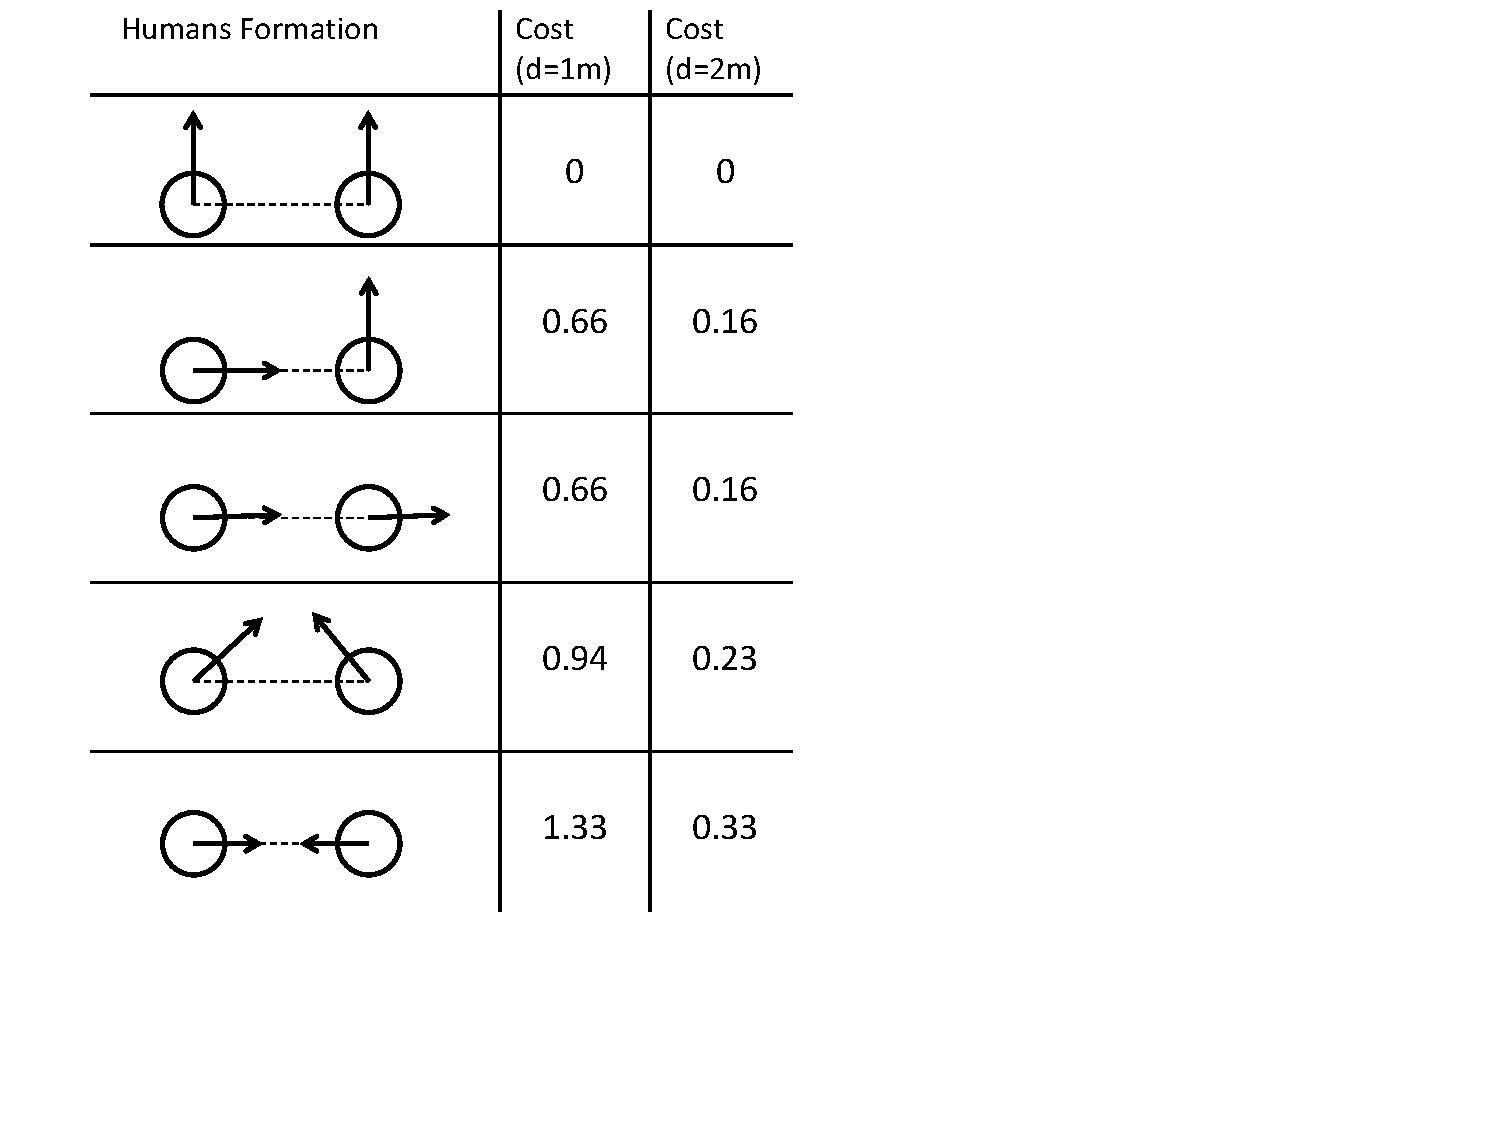
\includegraphics[width=0.4\textwidth]{pics/disturbance_ex_crop}
        }        
    \caption{%
	Disturbance costs in different human-human configurations and distances. A path that crosses the dashed lines incurs the disturbance cost calculated on the right side.
     }%
   \label{fig:sim}
   \vspace{-0.2cm}
\end{figure}



\textbf{Total Cost:} The total cost of a path $P$ is computed with a weighted average of path length, safety and disturbance costs. We use A* search to find the least-cost path.
\begin{align}
Cost_{Total}(P) = Cost_{path}+w_{s}.Cost_{safety} + w_d.Cost_{dist}
\end{align}

\subsubsection{Path Refinement using Social Forces}
\label{sec:navigation_path_refinement}

In this section, we describe the path refinement process that is applied to the global path. The initial geometric path generated by the global planner is not smooth, therefore robot motion might not be easy to interpret for human observers. The path refinement processes the global plan and simulates the parts of the path where group of humans are closeby. We use Social Forces Model (SFM) \cite{helbing1995social} to simulate the motions of both humans and the robot. Interaction between people are modeled as attractive and repulsive forces in SFM, similar to the Potential Field Method \cite{khatib1986real} for robot navigation. The forces are recomputed iteratively and the resulting simulated paths replaces the corresponding path sections in the global plan.

First, groups of people are found by clustering with respect to their positions. Simple euclidean distance thresholding is used for clustering. In our current implementation, a group region is defined as a rectangle, although other shapes are also possible. The path refinement process receives the global plan and finds out where it enters and exits each group region if it intersects the region. Goal of the dynamic iterative simulation is to find a sub-plan between those two points. Forces apply to all agents, including the robot and humans. We define 4 forces acting on the agents:
\begin{itemize}
  \item $F_{goal}$ : attraction towards a sub-goal
  \item $F_{social}$ : repulsion from other agents
  \item $F_{obs}$ : repulsion from nearest obstacle
  \item $F_{group}$ : attraction or repulsion towards group members
\end{itemize}
The forces acting on the robot at the first iteration of forces simulation are illustrated on the robot in Figure~\ref{fig:forces_robot}. The force magnitudes with respect to distances between entities are plotted in Figure \ref{fig:socialforces}. 

\begin{figure}[ht!]
\centering
%
        \subfigure[]{%
            \label{fig:forces_robot}
            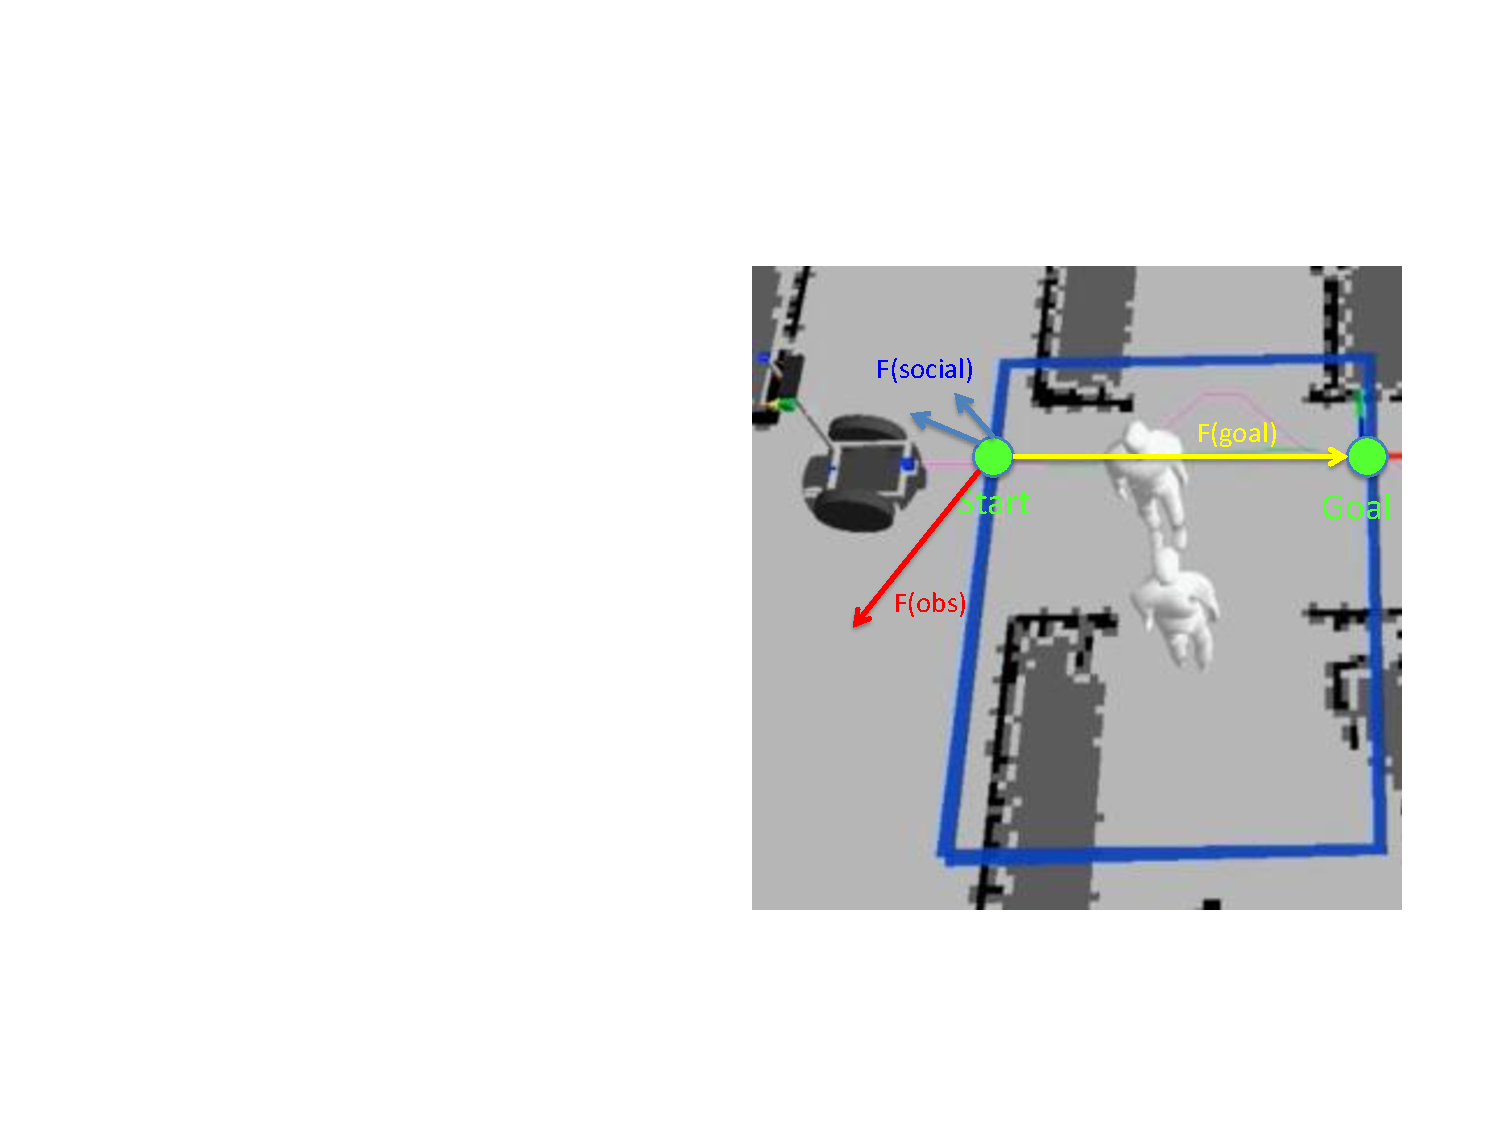
\includegraphics[width=0.43\textwidth]{pics/forces_robot_crop}
        }%
        \subfigure[]{%
           \label{fig:socialforces}
           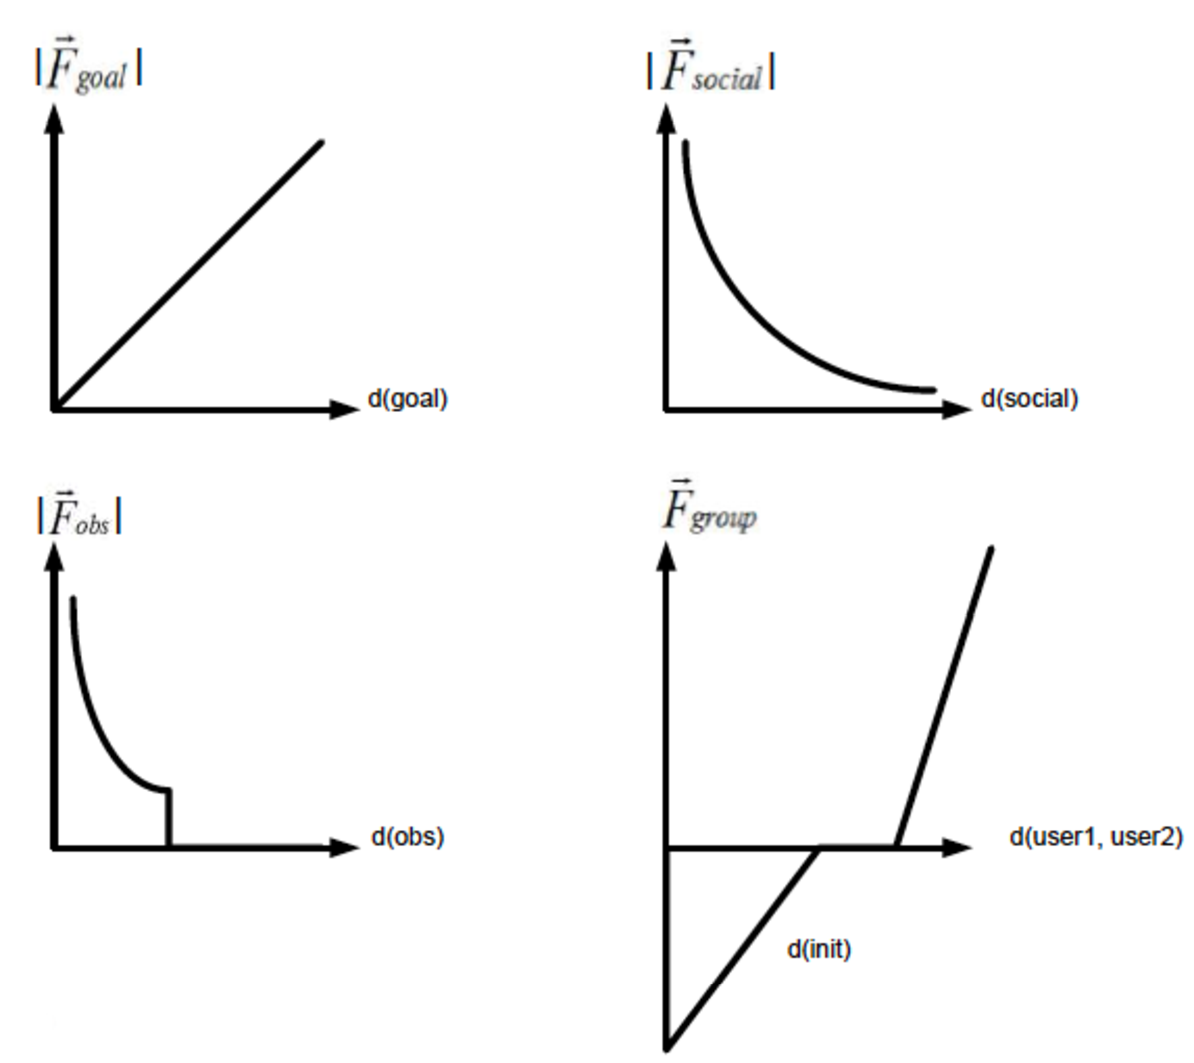
\includegraphics[width=0.53\textwidth]{pics/socialforces}
        }        
    \caption{%
	a) Social forces acting on the robot, including $F_{goal}$,$F_{social}$,$F_{obs}$, are shown at the first iteration of the dynamic planner. Note that $F_{group}=0$ as the robot does not belong to a group. The group force (not shown) exists, however, for the humans as they are in the same group region. b) Social forces with respect to the distance towards the corresponding entity.
     }%
   \label{fig:forces}
\end{figure}


Starting from the first group region that intersects the static plan, the following procedure is applied within every group region: At every iteration, first the resultant force vector acting on the robot is found. Then the planner takes a step in the direction of the $F$ vector for a fixed step size. Then each of the humans in the group takes a step towards the resultant force that is acting on them. The planner continues the iterations until a solution is found. If a solution is found, the calculated sub-plan replaces the static plan in this group region. Potential fields are known to stuck to local minima~\cite{koren1991potential}, and the planner might go into infinite loop. We stop the planner after a number of iterations and accept the static plan in the corresponding group region if that happens.

We assume that humans have a cognitive model of the robot, by thinking that the robot has a limited Field of View (FOV). When the robot has gone past a human (out of the FOV), then we make the repulsion force $F_{social}=0$. We think that humans behave that way: as someone walks past, there are no social constraints resulting from that individual any more.

\subsection{Local Planner}
\label{sec:navigation_local_planner}

The local planner is responsible for finding the trajectory that the robot is capable of executing. It accepts a geometric global path as input and computes the linear and angular velocity necessary to follow the dynamic path. We adopt a local planner inspired by Dynamic Window Approach (DWA) by Fox \cite{fox1997dynamic}. In the original DWA approach, only circular trajectories are considered, defined by pairs $(v,w)$ of linear and angular velocities. An objective function, consisting of target heading, clearance from obstacles and velocity of the robot is maximized by sampling admissible velocities.

Our approach also samples admissible velocities, but the optimization criteria we use consists only of the Euclidean distance to a sub-goal point chosen on the path that is ahead of the robot. The velocity pair that resulted in the closest proximity to the sub-goal is chosen and sent to robot controllers. At every control iteration, the sub-goal is chosen as the first point ahead of the robot that is further than a distance threshold. We found that a threshold of 0.25 meters was sufficient to choose the sub-goal. After the local planner calculates the output velocities, they are applied to the robot and the iterative process continues until the the robot reaches the goal. Since the goal is a singular point, it is impossible for the robot to be exactly at the goal. Therefore, a tolerance around the goal point, defined as a circle around the goal is defined.

Given the robot's current pose and an applied velocity, the DWA approach requires to have a motion model for the robot. The motion model projects the what the robot pose would be, if a velocity pair is applied to it for a time period. The robot we used for our implementation is a non-holonomic two wheeled robot. While one can use the general motion equations derived in \cite{fox1997dynamic}, we used linear approximated motion equations for our robot in Equation \ref{eq:motion_model}. Given a robot pose $q^t=(x^t,y^t,\theta^t)$ at time $t$ and an input velocity $(v,w)$, the projected robot pose at time $t+\Delta t$ is:

\begin{align}
q^{t+\Delta t} = 
f_{motion}(q^t,v,w,\Delta t) =
\begin{Bmatrix}
x^t-\frac{v}{w}sin(\theta^t)+\frac{v}{w}sin(\theta^t+w \Delta t)\\
y^t+\frac{v}{w}cos(\theta^t)-\frac{v}{w}cos(\theta^t+w \Delta t)\\
\theta^t + w\Delta t
\end{Bmatrix}
\label{eq:motion_model}
\end{align}


%We use  for obstacle avoidance of non-holonomic robots. (TODO: DWA our version, derive motion model, vs. ) DWA samples linear and angular robot velocities and simulates the robot trajectory for each of them. First, a waypoint on the dynamic path is chosen as a sub-goal. At every control iteration, the waypoint is chosen as the first point ahead of the robot that is further than a distance threshold. We found that a threshold of 0.25 meters was sufficient. Robot is simulated with each velocity combination and the trajectory that gets closest to the sub-goal is sent to the motor controllers.

\subsection{Results}
\label{sec:navigation_results}

In this section, we provide qualitative results both in simulation and on the real robot. We used a non-holonomic drive robotic platform, Segway RMP-200, for the real experiments. We used our laser-based torso tracking method presented in Section \ref{sec:multimodal_torso_detection}.

\subsubsection{Simulation}
\label{sec:navigation_results_simulation}

\begin{figure}[h!]
\centering
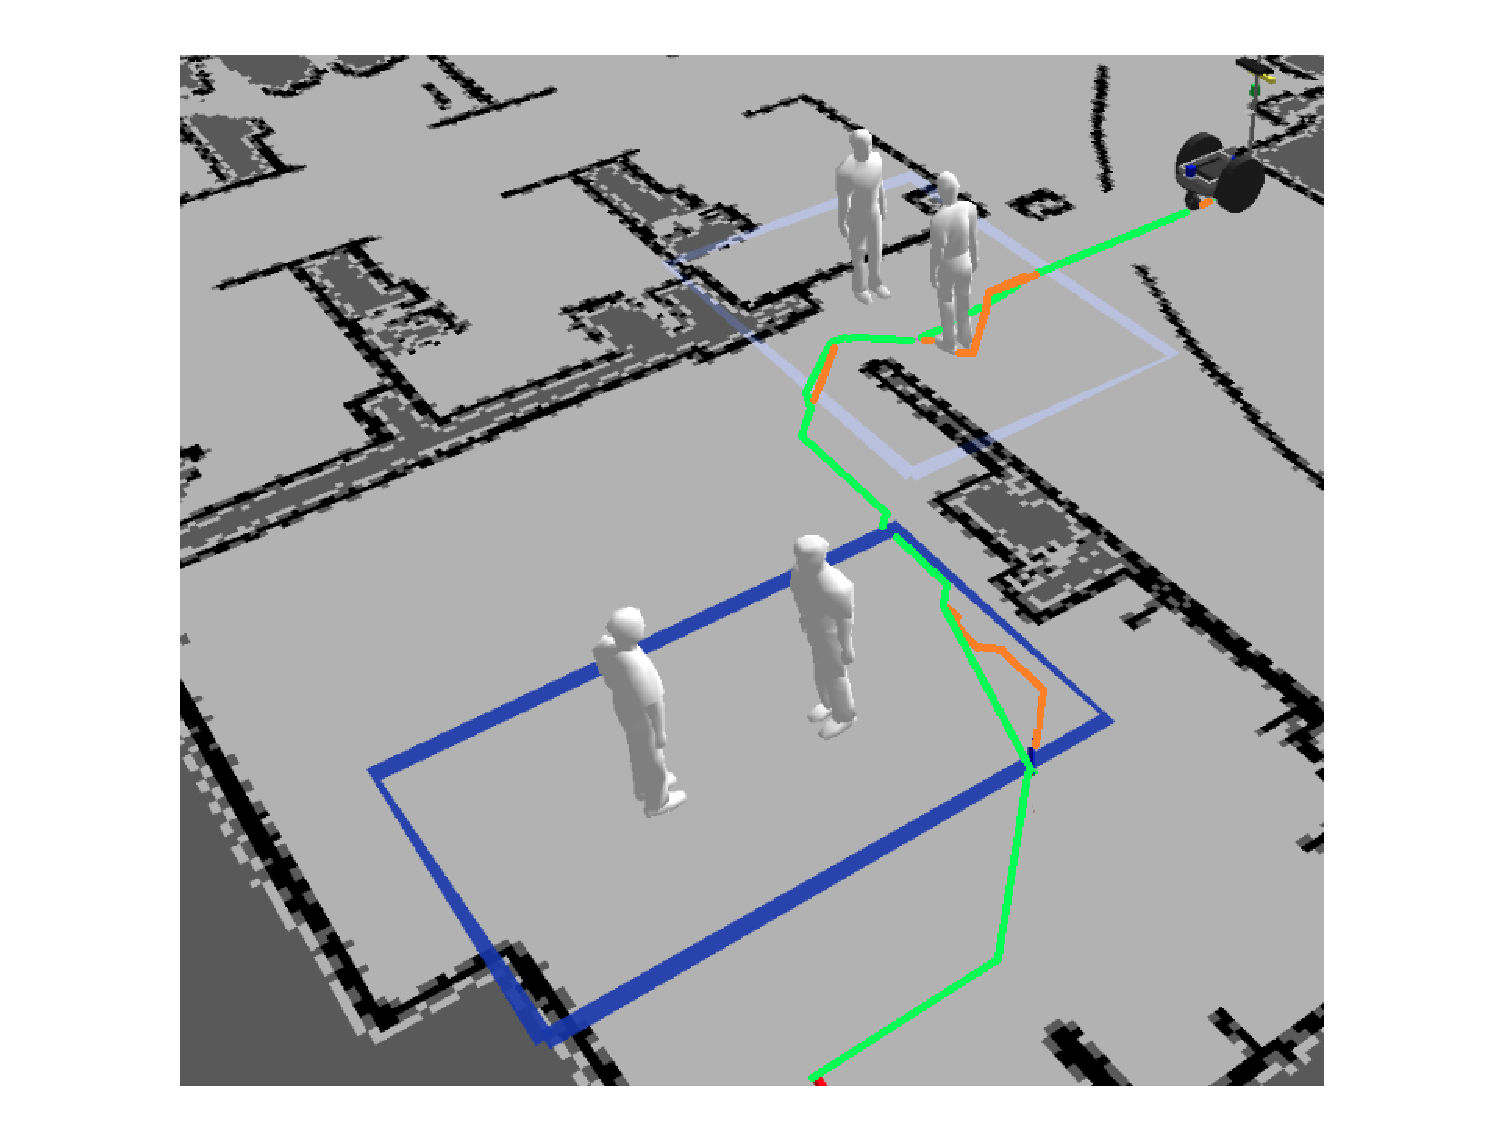
\includegraphics[width=0.5\textwidth]{pics/room_sol_crop}
\caption{"Room Problem". The robot is outside a room and the goal is inside the room. Traditional planners can not solve the problem because two people are blocking the doorway. Our planner generates a tentative path, with the initial global plan shown in green and the dynamic refinements are shown in orange.}
\label{fig:room_sol}
\end{figure}

\begin{figure}[hbtp]
\centering
        \subfigure[]{%
            \label{fig:sim2}
            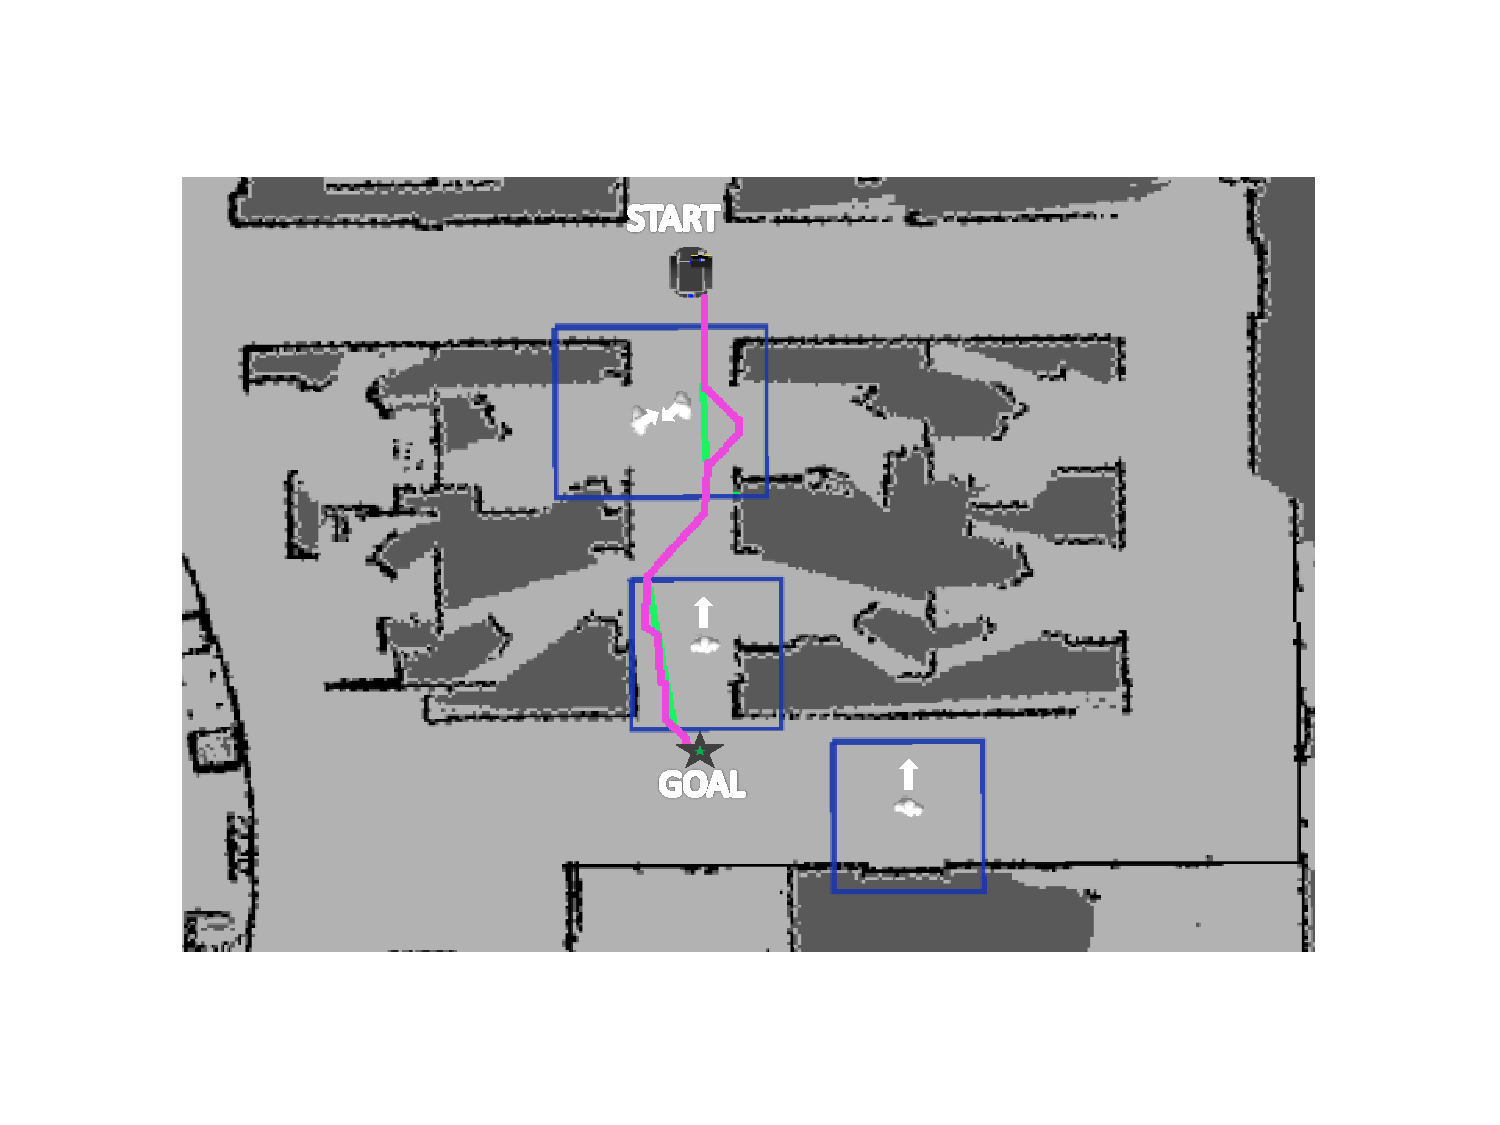
\includegraphics[width=0.6\columnwidth]{pics/sim2_crop}
        } \\
        \subfigure[]{%
           \label{fig:sim3}
           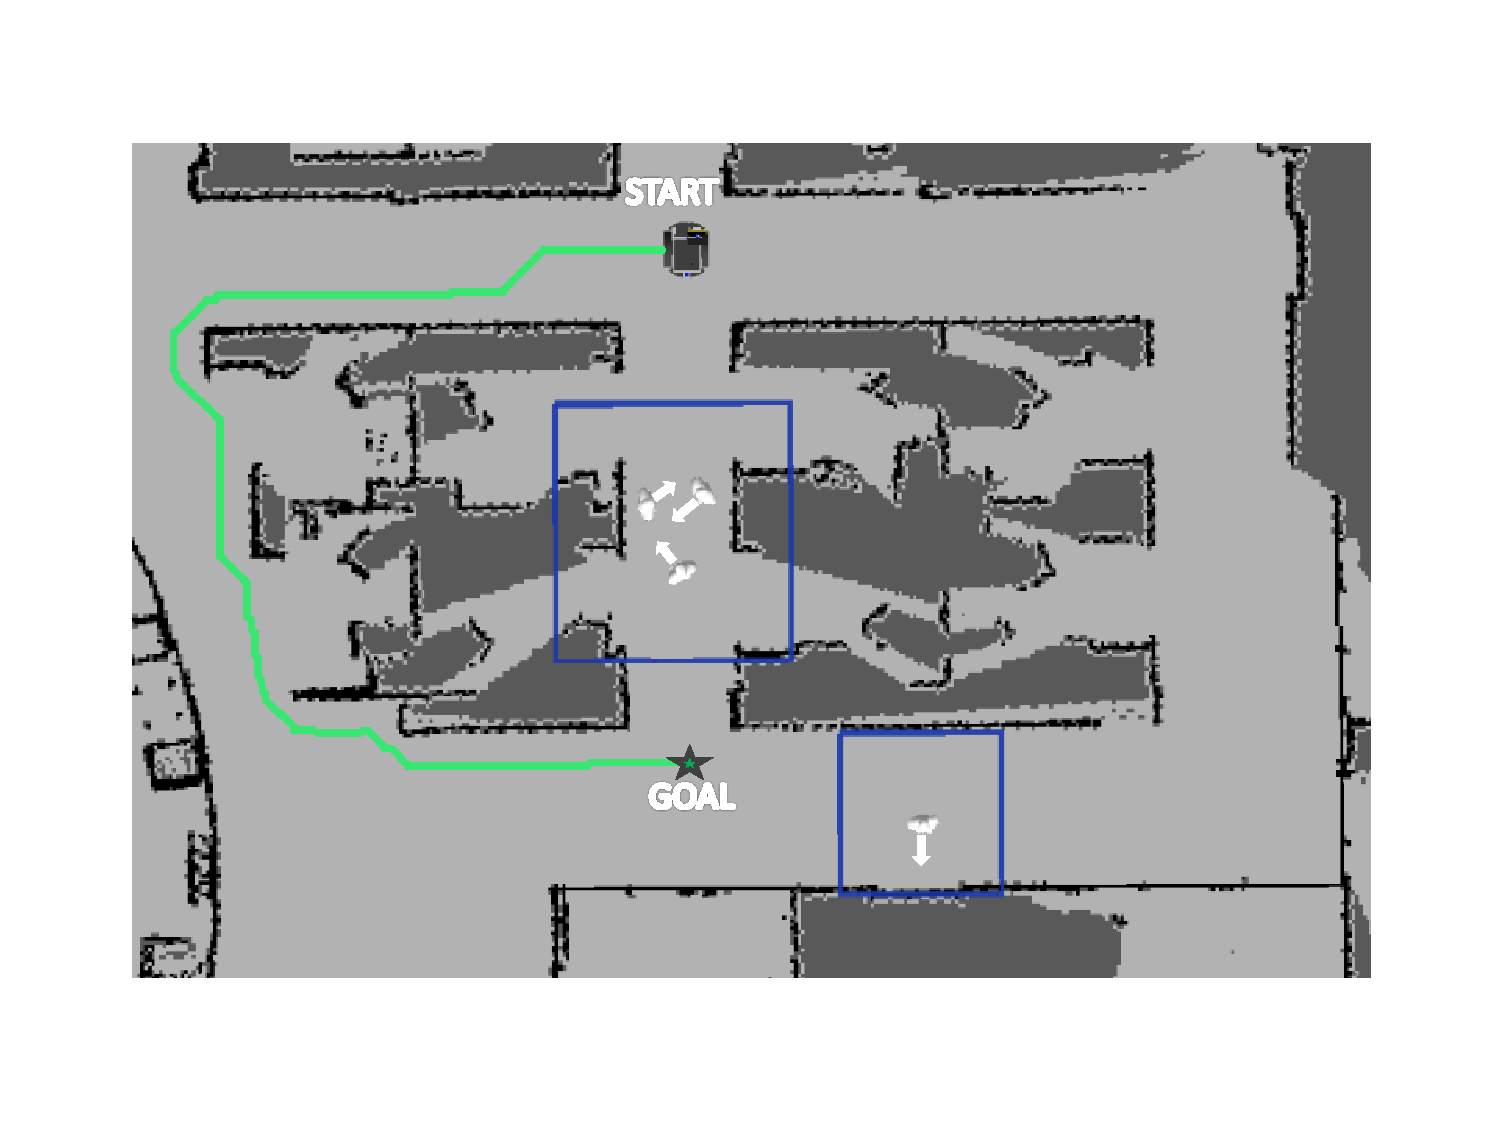
\includegraphics[width=0.6\columnwidth]{pics/sim3_crop}
        }
	\subfigure[]{%
           \label{fig:sim1}
           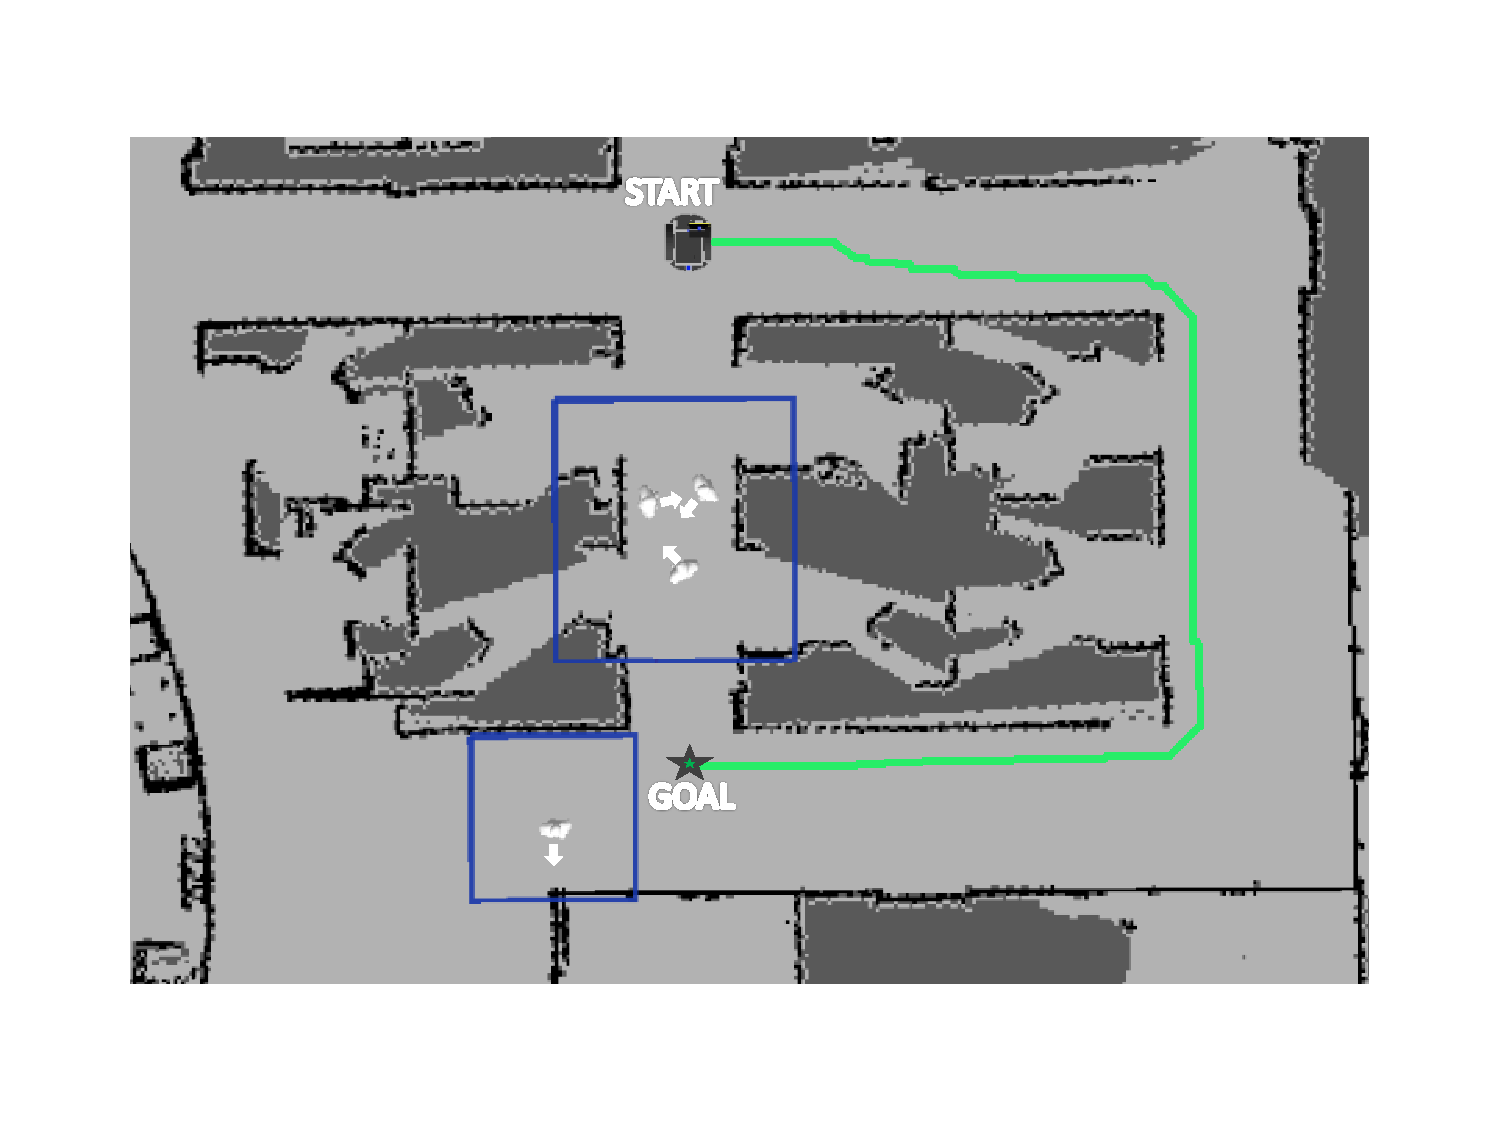
\includegraphics[width=0.6\columnwidth]{pics/sim1_crop}
        }        
    \caption{%
	Paths differ drastically with the poses and grouping of humans. a) The robot takes shortest route, traveling in the vicinity of a group of two and another individual. b) third individual joins the group. Robot takes a longer path that doesn't have humans on path. c) fourth person changes his position, leading the robot to take the longest route.
     }%
   \label{fig:sim}
\end{figure}


\textbf{Room Problem: } In this scenario, the robot is outside the room and a point inside the room is given as the goal (Figure~\ref{fig:room_sol}). Traditional planners can not return a solution in this scenario because there is not enough space for the robot to navigate inside. There are two people standing at the doorway and there are two more standing people inside. The static plan and dynamic plans are shown in green and orange, respectively. This path is planned for the current time but makes assumptions about future positions of humans. Note that the dynamic planner modifies only the parts of plan inside group regions (blue rectangles). In the first group region (doorway), the static plan involves going between the humans. Dynamic simulation suggests that people will get closer to each other if the robot drives towards the side. In the second group region, since two humans are oriented to each other, going between them would add a high disturbance cost, therefore the static plan avoids going between them. Safety costs encourages staying far from the humans, but not too far because a longer path would increase the path length cost. The robot is further led to stay closer to the room boundaries in the dynamic planner due to the repulsive forces from both humans.




\textbf{Office Environment: } Goal of the robot is to navigate to a goal position in an office environment with 4 standing people (Figure~\ref{fig:sim}). In this scenario, we show how the planned path is drastically changing with the poses of humans even though the start and goal position of the robot doesn't change. There are 3 main ways the robot can navigate to its goal: left, center or right corridor. 

In the first configuration in Figure~\ref{fig:sim2}, two people are grouped together as they are looking at each other and likely conversing. The robot decides to take the center corridor, first slightly disturbing the speaking duo, then switches sides in the corridor and reaches its goal. In the figure, the dynamic path (pink line) is overlaid on the static path (green line). 

In the second configuration in Figure~\ref{fig:sim3}, The third person at the center corridor joins the conversation. Now we have 2 group regions (rectangles) in the scene. Since passing through a group of 3 people would introduce a high disturbance cost in addition to the safety cost, the robot decides to take a longer route (left corridor). Since this path does not intersect any group regions, no dynamic simulation is done.

In the third configuration in Figure~\ref{fig:sim1}, the group of three hasn't moved, but the fourth person person has changed its position. In this case, if the left corridor is taken again, an additional safety cost would be incurred. Therefore the robot decides to take the longest route (right corridor). Again, since the robot travels far from humans, no dynamic simulation is done.

\subsubsection{Real Robot}
\label{sec:navigation_results_real_robot}


We demonstrate our anticipatory navigation planner on the real system in two environments: hallway and kitchen. Each scenario is run twice under different human positions and behaviors in order to show how the planner responds.

\textbf{Hallway passing: } In this scenario (Figure~\ref{fig:corridor}), robot's goal is to navigate to the end of the hallway. In the first run, humans move as the robot anticipates. In the second run, humans do not move as anticipated, and the robot adjusts its path. Each step is described in the caption of the figure. In both cases, the initial plan is to disturb the interaction by going between the two. This is because the safety cost for getting close to one of the humans was more dominant than the disturbance cost.

\textbf{Narrow corridor:} In this scenario (Figure~\ref{fig:kitchen}), robot's goal is to drive towards the exit door. There are 3 people nearby the robot. The robot can either take the shorter route that is the direct path, or take a longer path that is to the left of the table. Each important step is described in the caption of the figure. The first run shows that the robot may plan hoping to influence the human. The second run shows that the robot may take a longer route if the disturbance and safety costs are going to be large.

\begin{figure}[p!]
\centering
%
        \subfigure[]{%
            \label{fig:corridor1}
            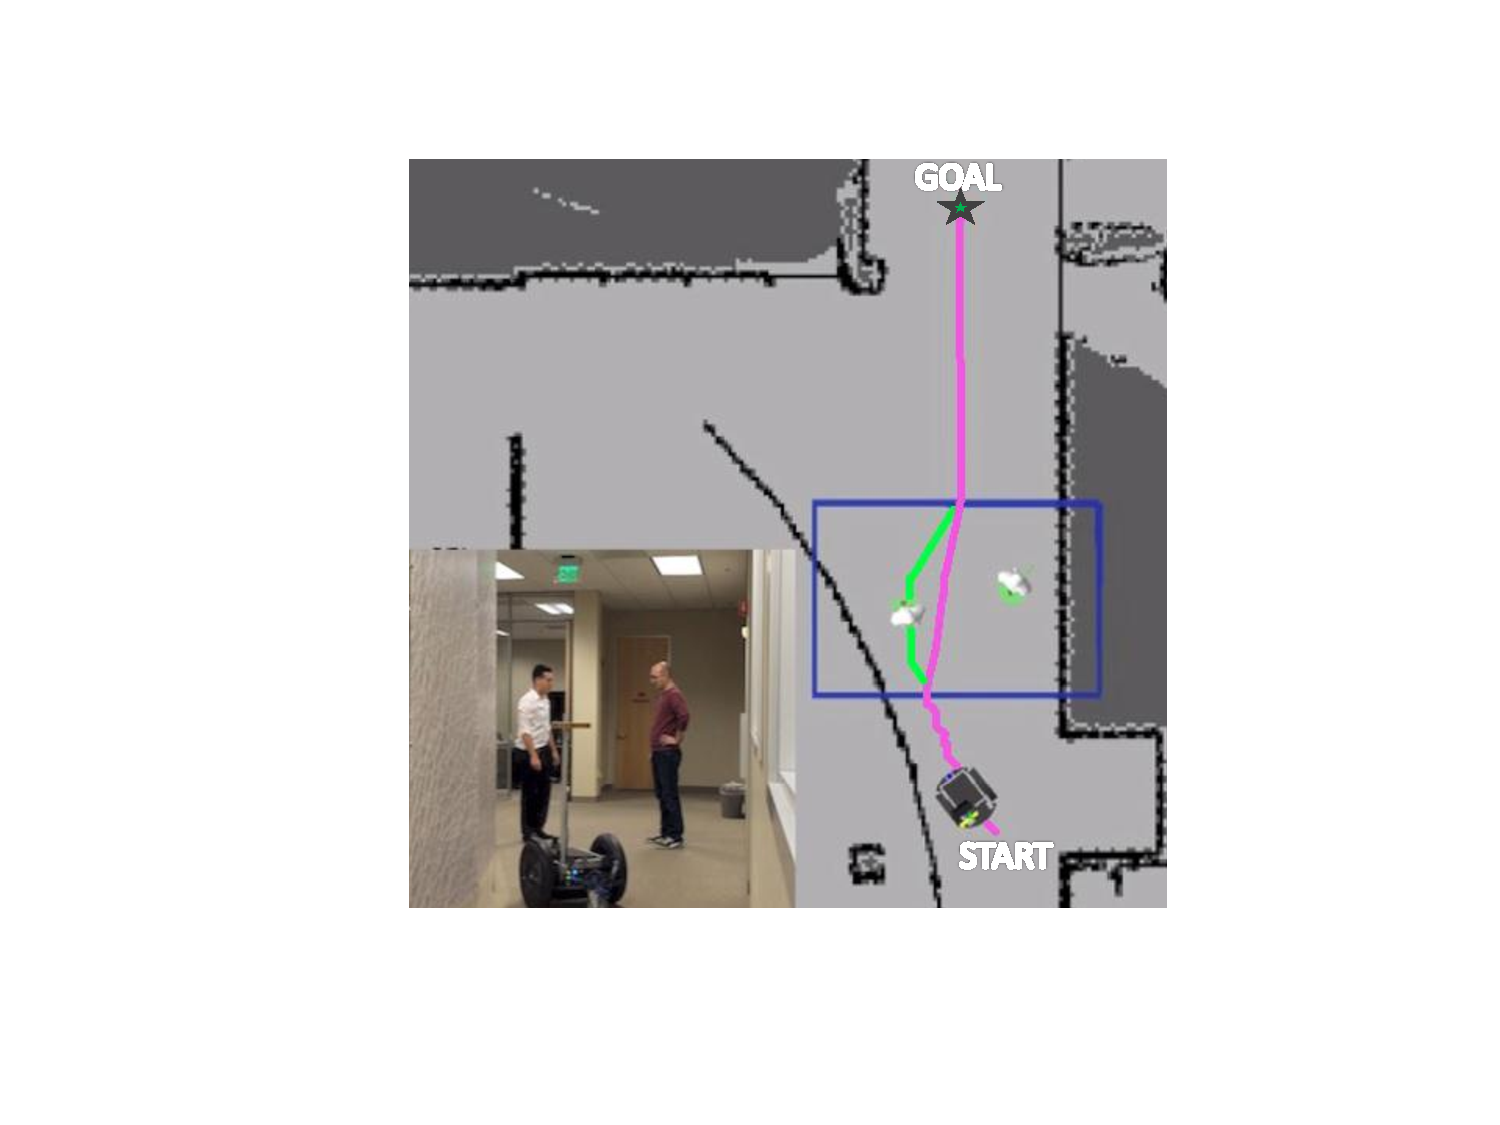
\includegraphics[width=0.58\columnwidth/2]{pics/corridor1_crop}
        }%
        \subfigure[]{%
           \label{fig:corridor2}
           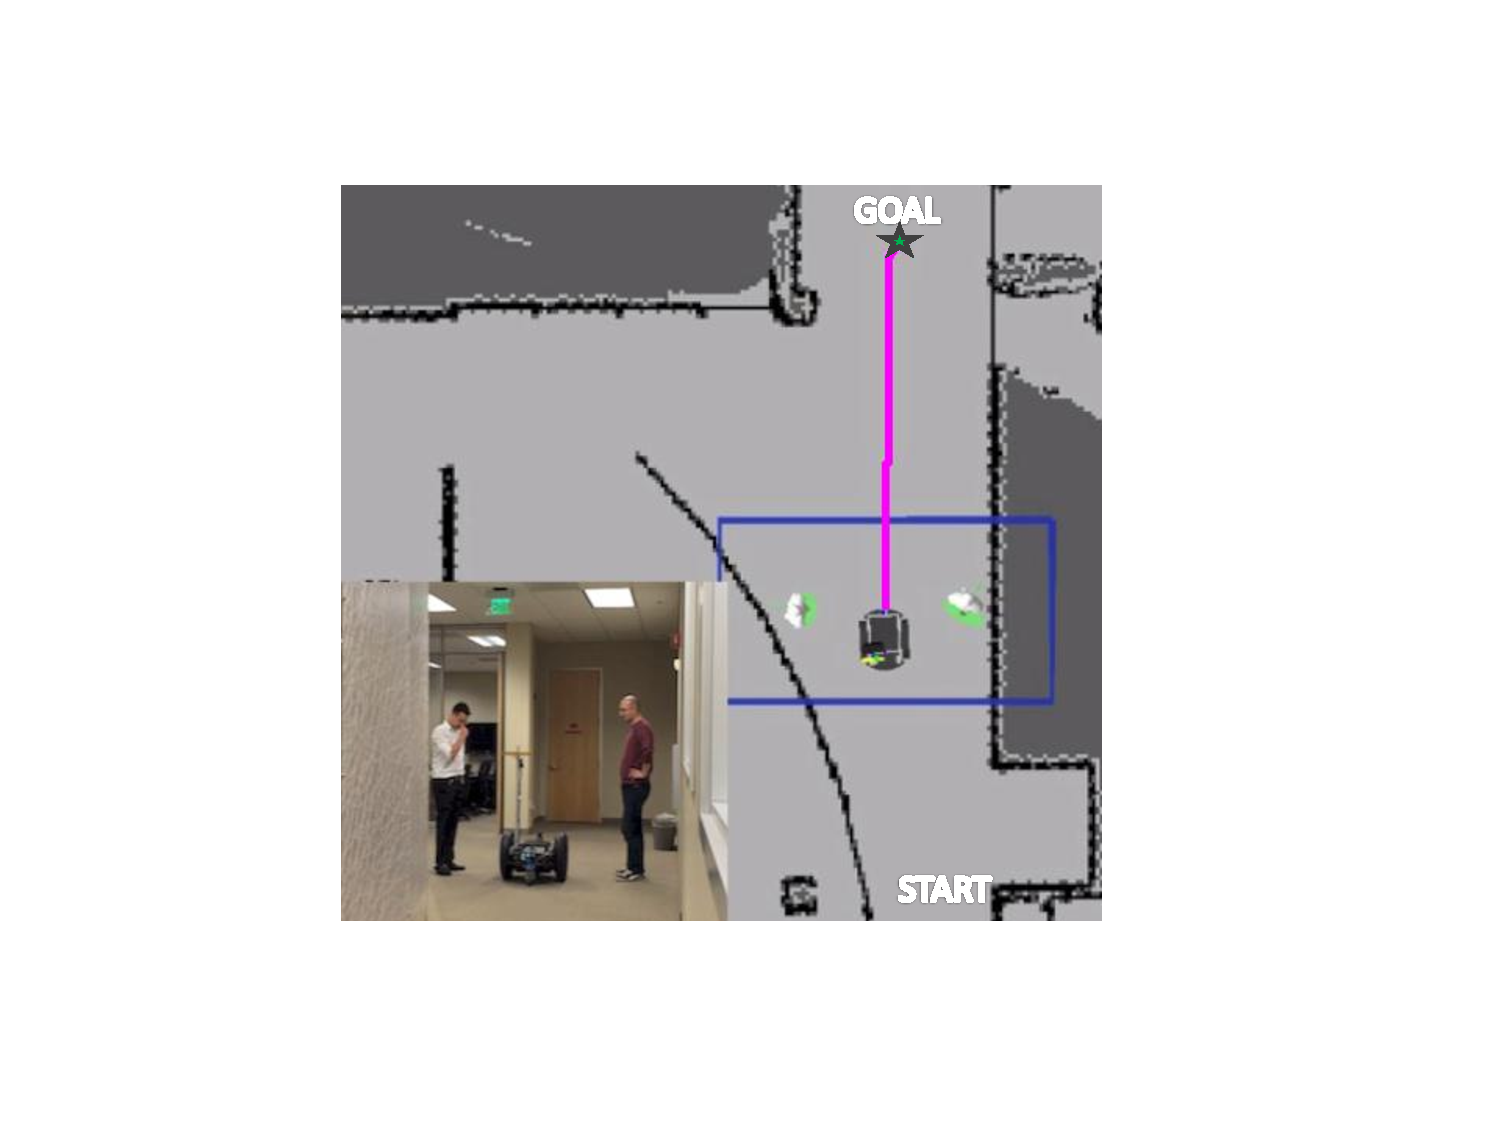
\includegraphics[width=0.58\columnwidth/2]{pics/corridor2_crop}
        }
        \subfigure[]{%
           \label{fig:corridor3}
           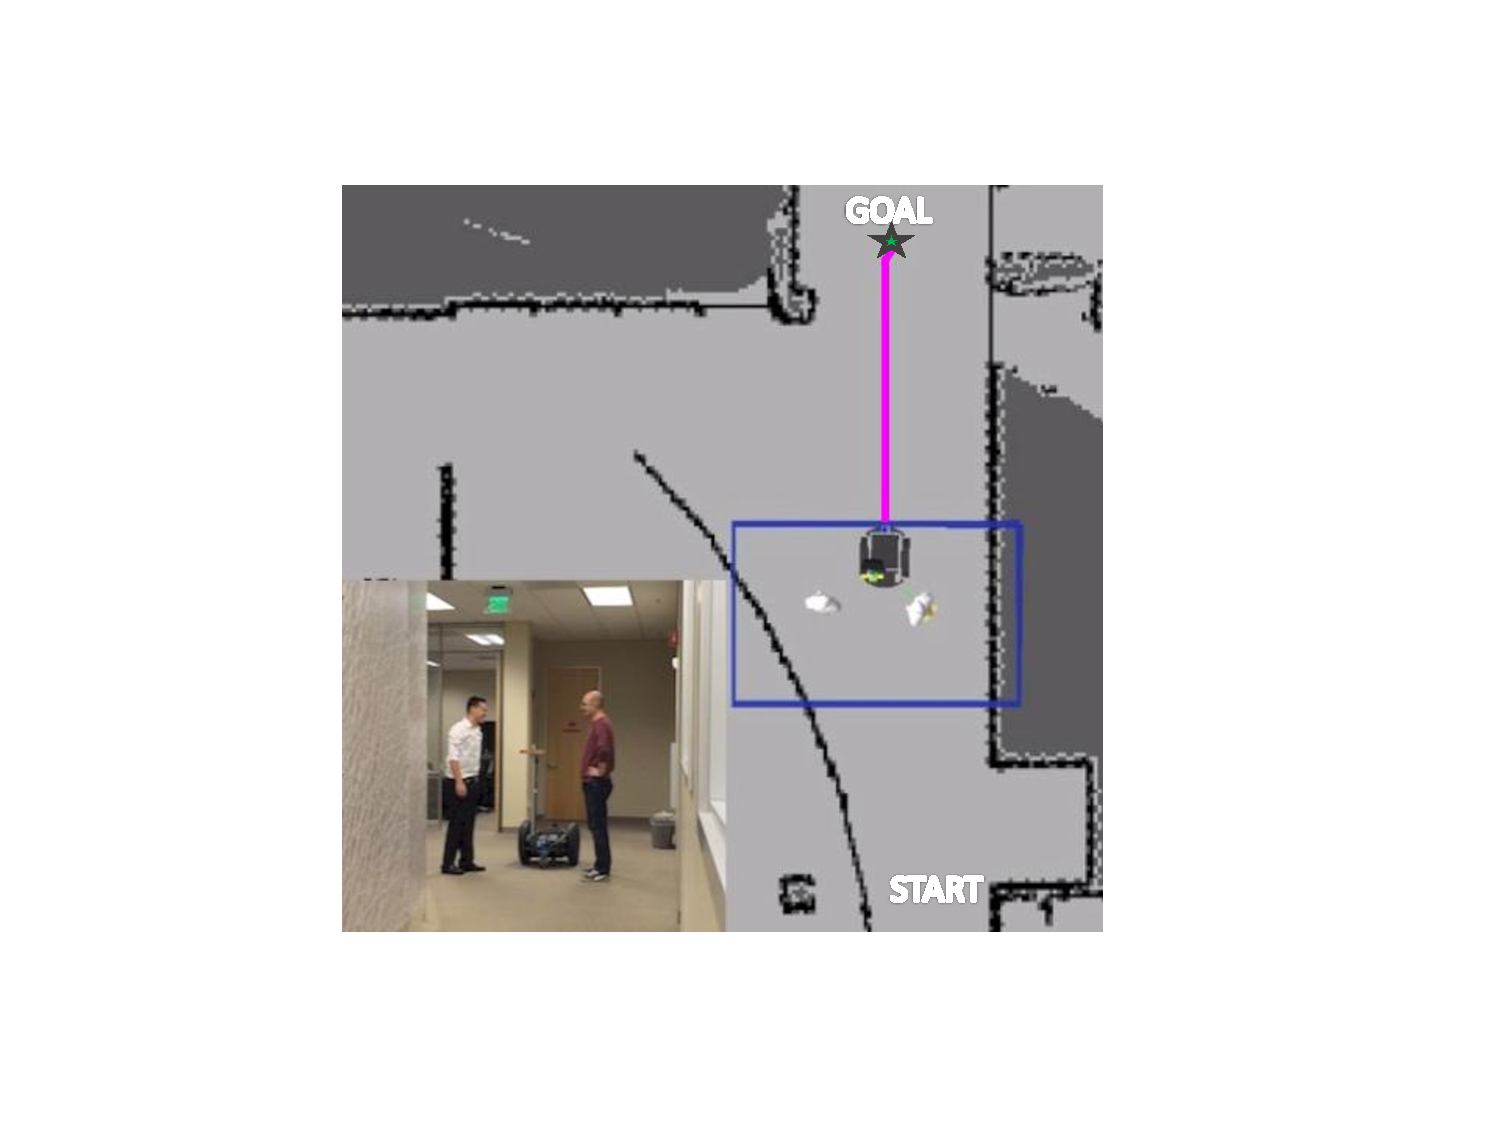
\includegraphics[width=0.58\columnwidth/2]{pics/corridor3_crop}
        }
\subfigure[]{%
           \label{fig:corridor4}
           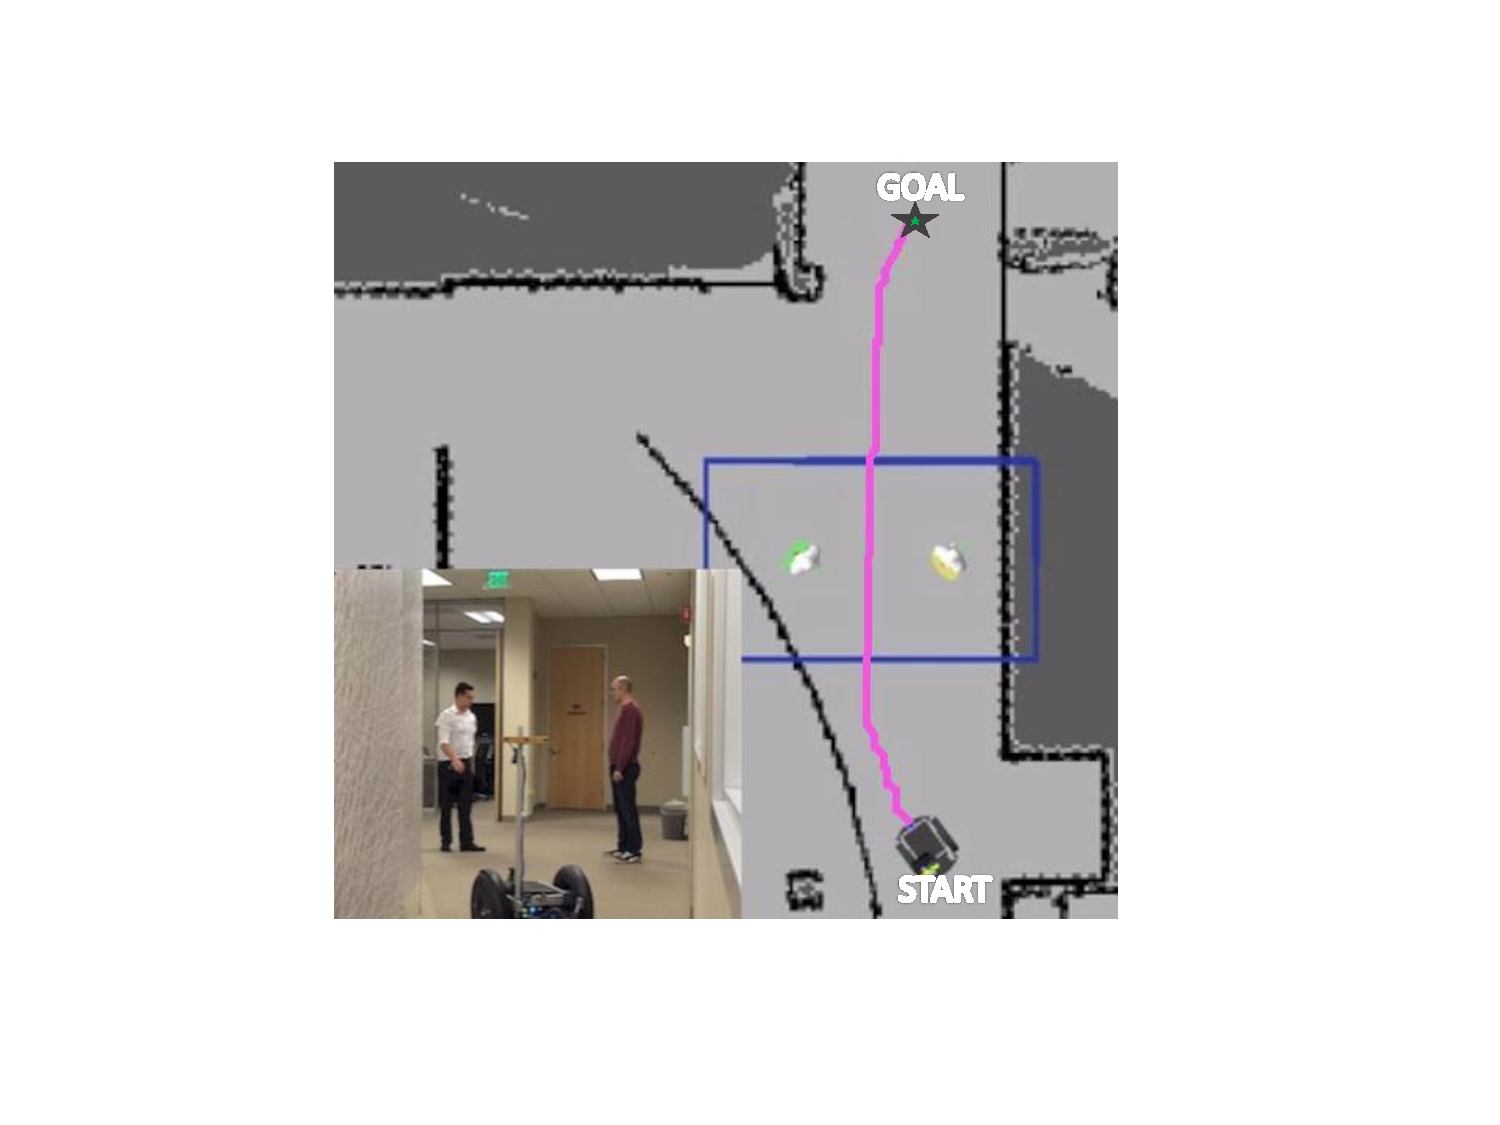
\includegraphics[width=0.58\columnwidth/2]{pics/corridor4_crop}
        }
\subfigure[]{%
           \label{fig:corridor5}
           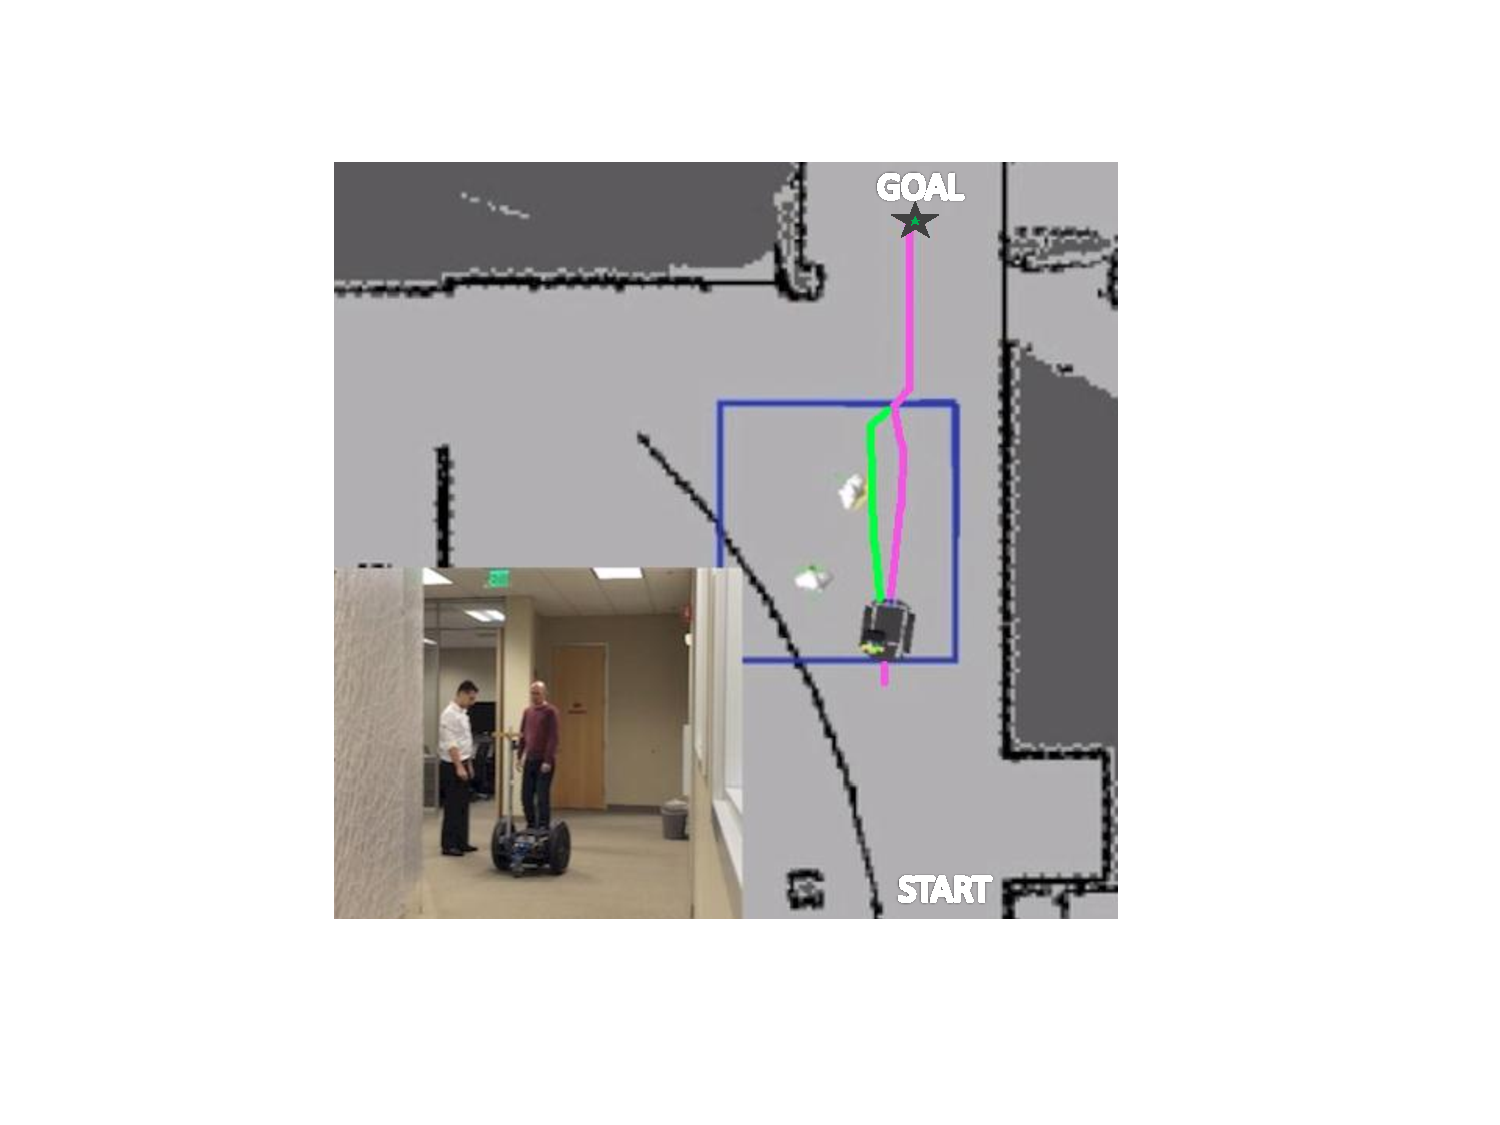
\includegraphics[width=0.58\columnwidth/2]{pics/corridor5_crop}
        }
\subfigure[]{%
           \label{fig:corridor6}
           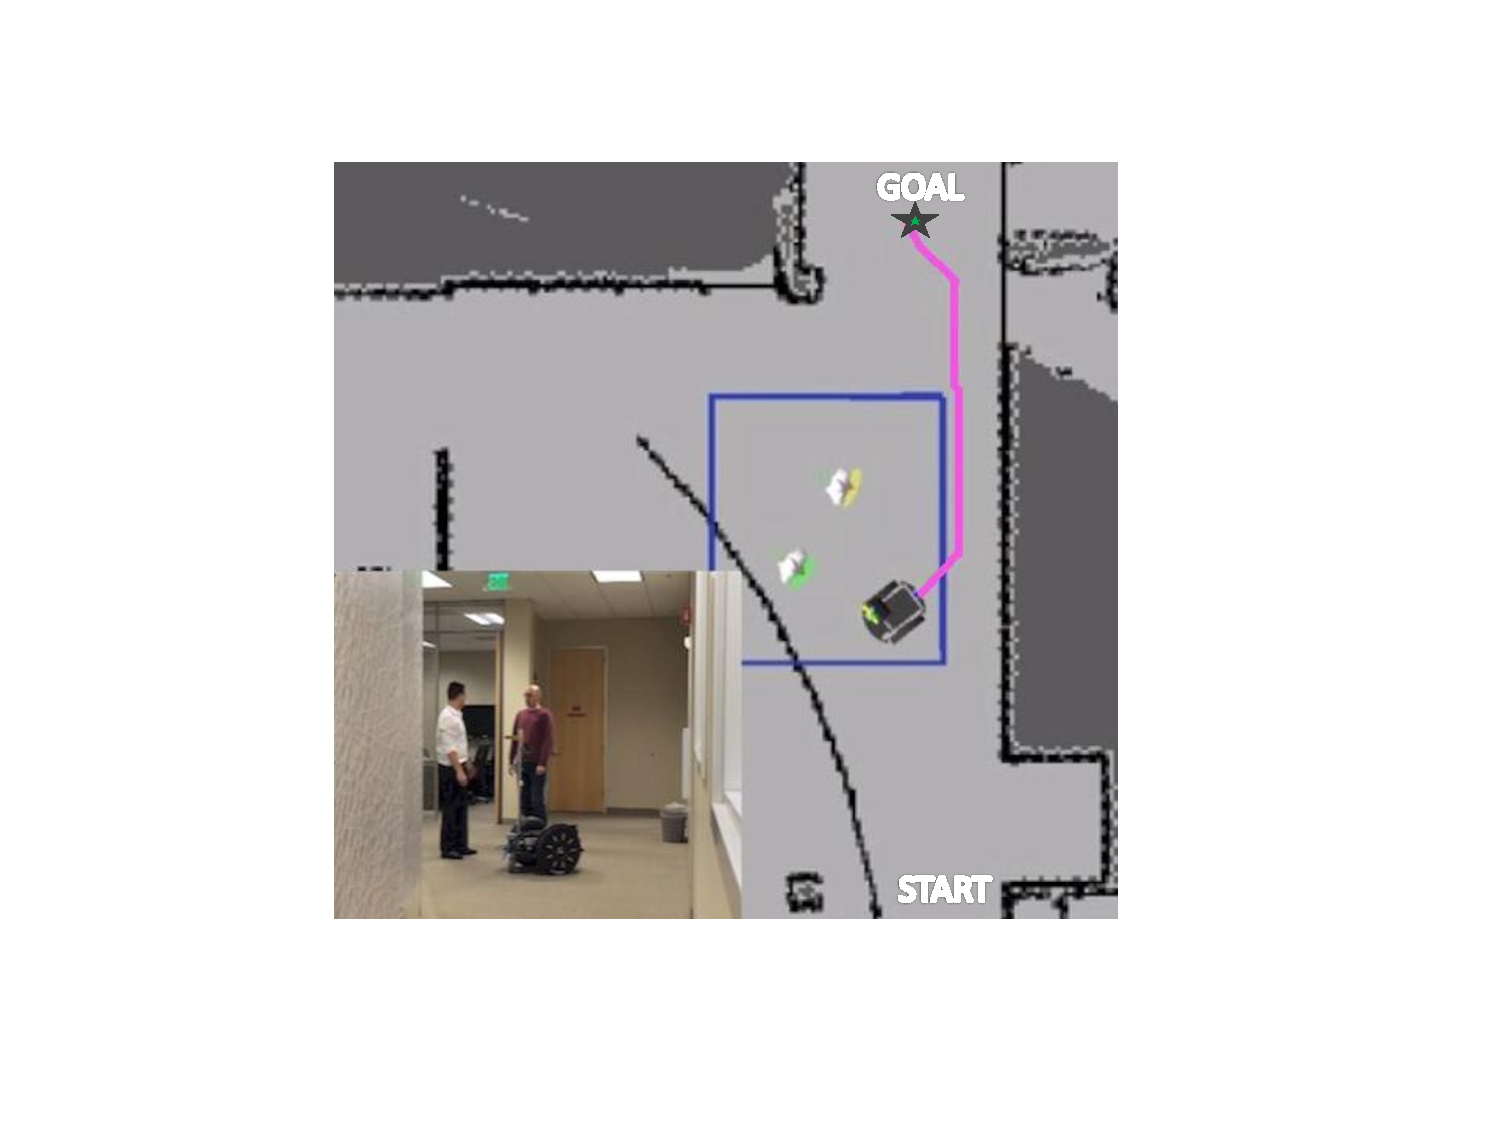
\includegraphics[width=0.58\columnwidth/2]{pics/corridor6_crop}
        }
    \caption{%
	The Hallway scenario. 2 runs are shown in first and second rows.The static plan (green line) and dynamic plan refinement (pink line) are shown. First run: a) Navigation starts. The dynamic planner anticipates that people will give way to the robot when it starts to move towards them. b) Humans notice the robot, and give way by increasing the separation between them. c) The robot continues towards its goal and humans regroup. Second run: d) both the static and dynamic plan involves going in between humans again e) human on the right gets closer to the other person. Since a human made significant movement, dynamic planner re-plans. Plan no longer involves going in between. f) static planner periodic re-plan triggers, leading to robot to stick to the wall to the right.
     }%
   \label{fig:corridor}
\end{figure}


\begin{figure}[p!]
\centering
%
        \subfigure[]{%
            \label{fig:corridor1}
            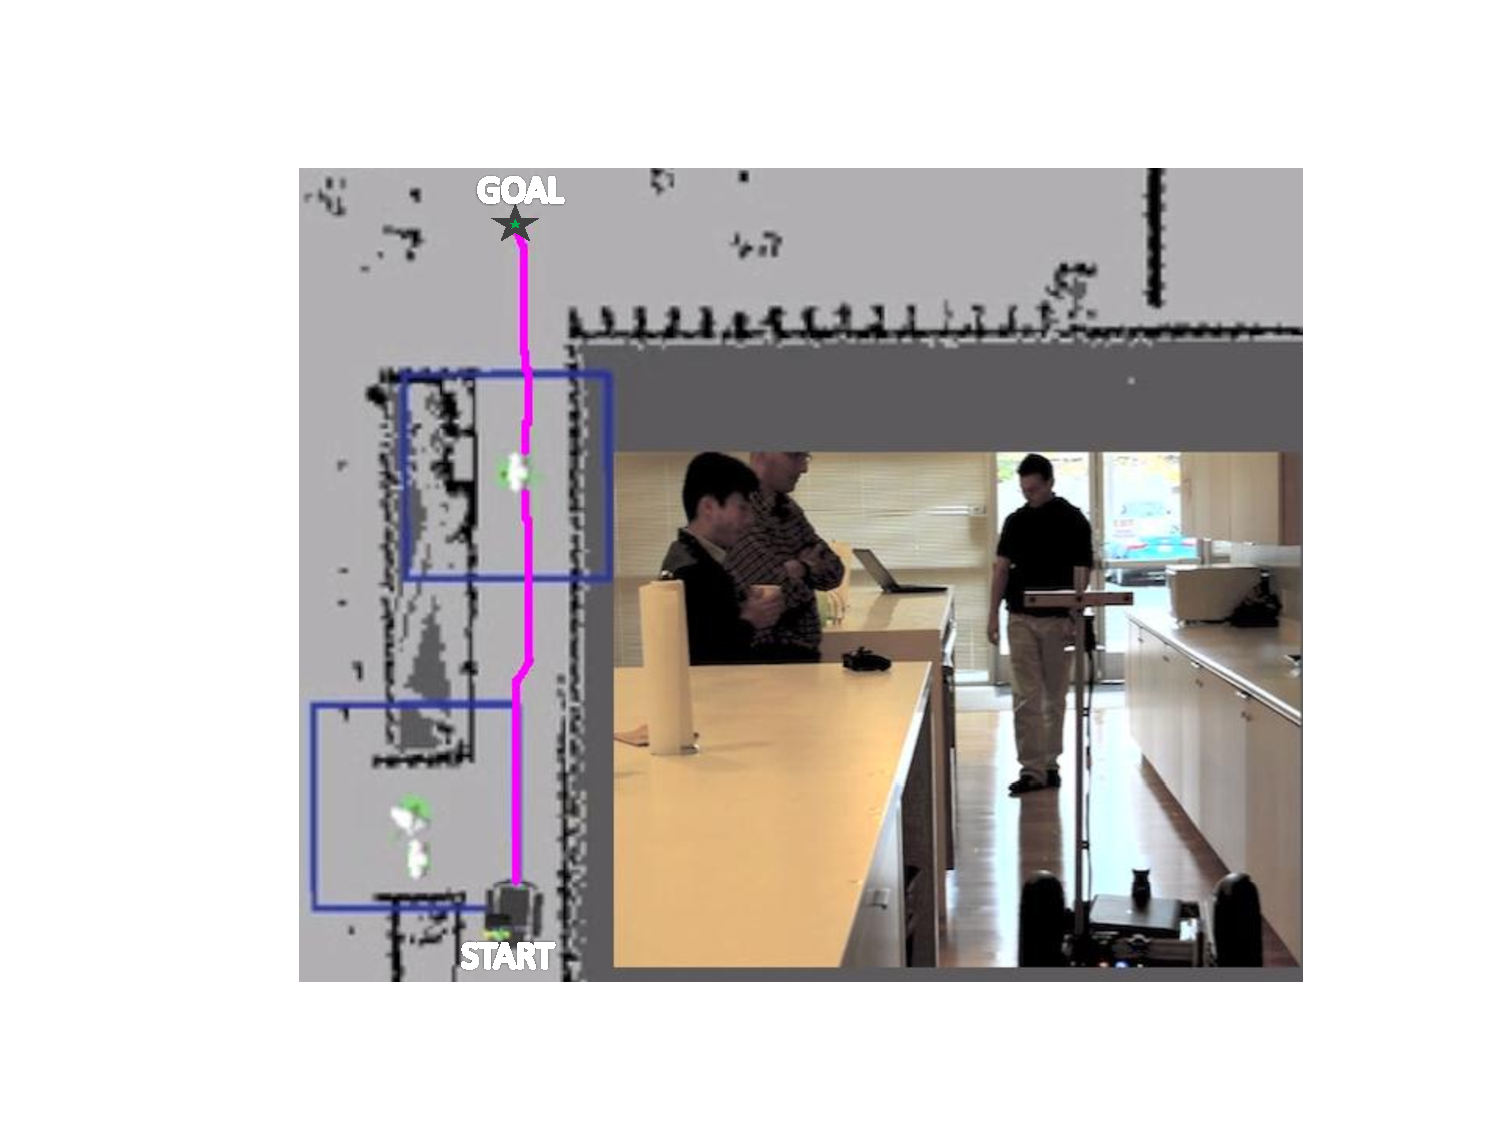
\includegraphics[width=0.6\columnwidth/2]{pics/kitchen1_crop}
        }%
        \subfigure[]{%
           \label{fig:corridor3}
           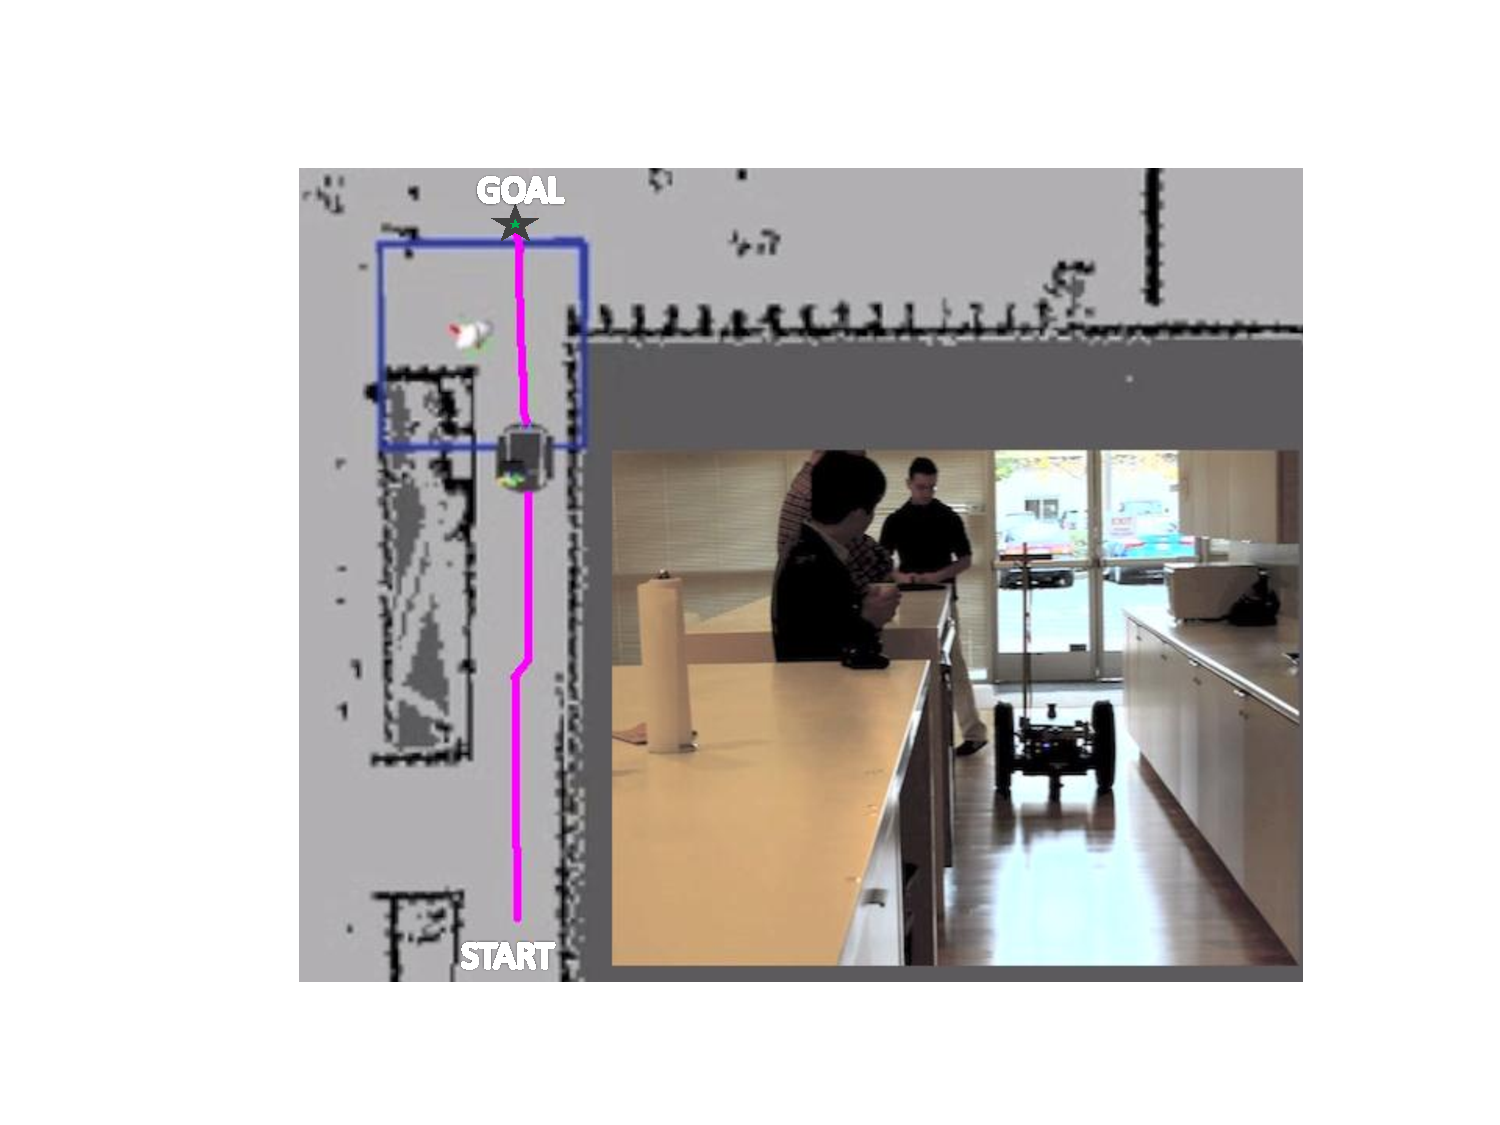
\includegraphics[width=0.6\columnwidth/2]{pics/kitchen3_crop}
        }
\subfigure[]{%
           \label{fig:corridor4}
           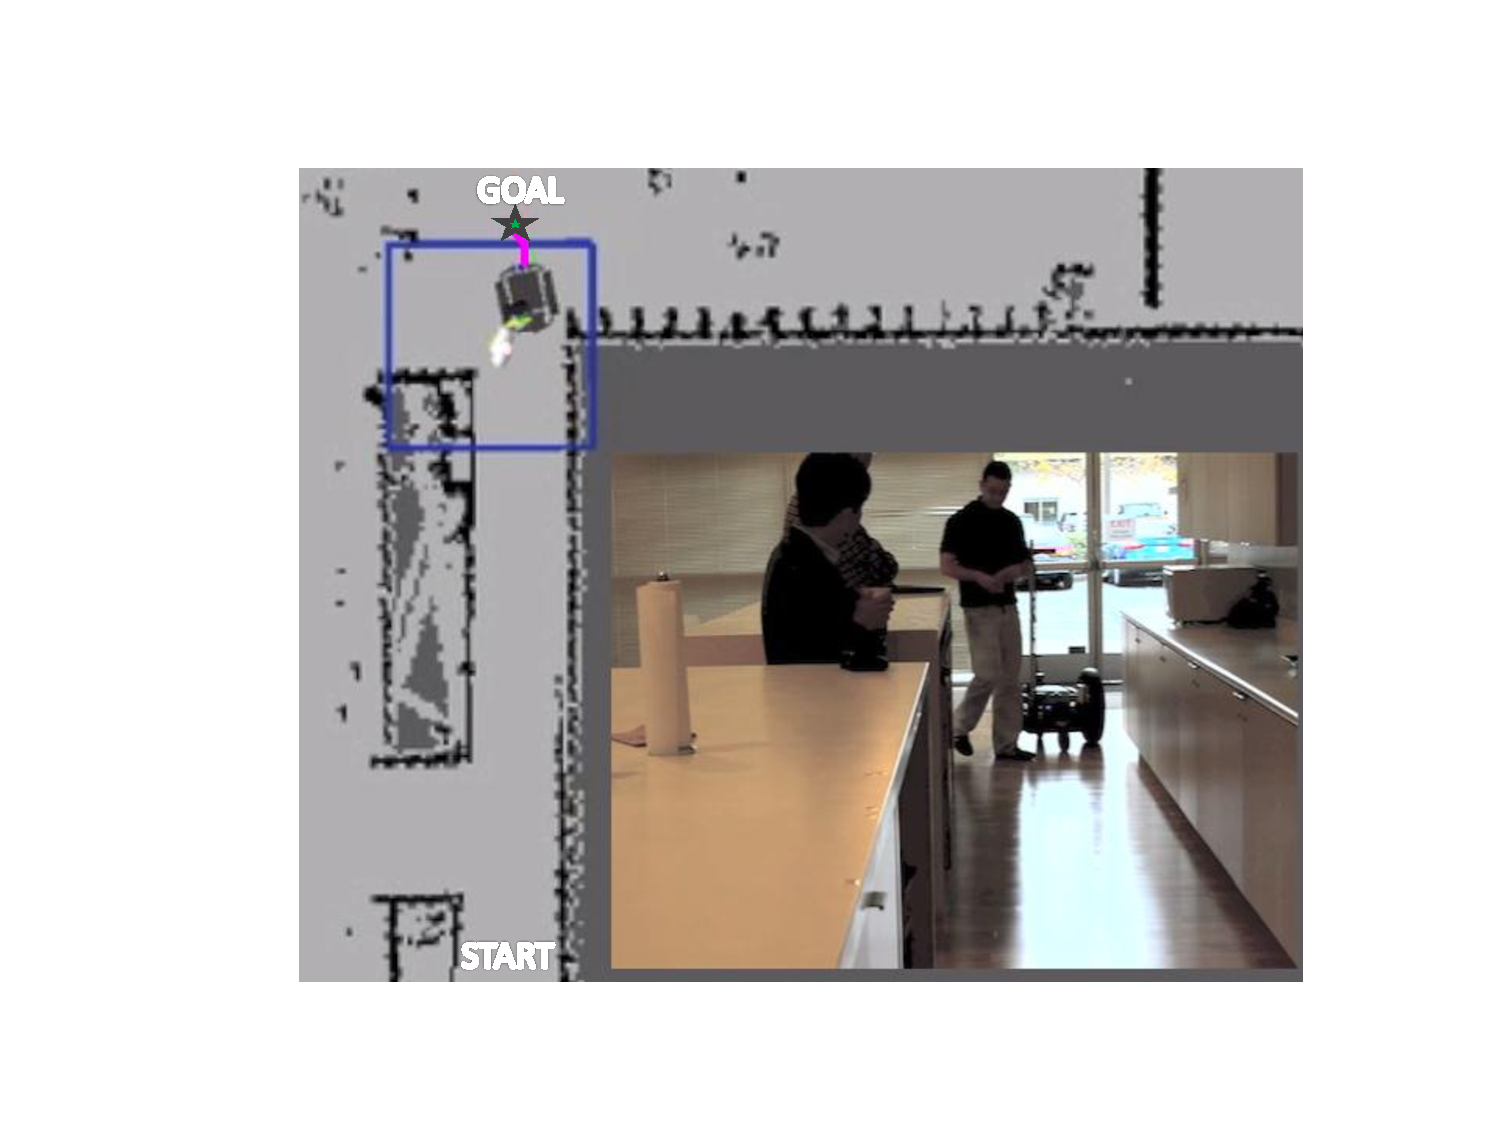
\includegraphics[width=0.6\columnwidth/2]{pics/kitchen4_crop}
        }        
\subfigure[]{%
            \label{fig:corridor1}
            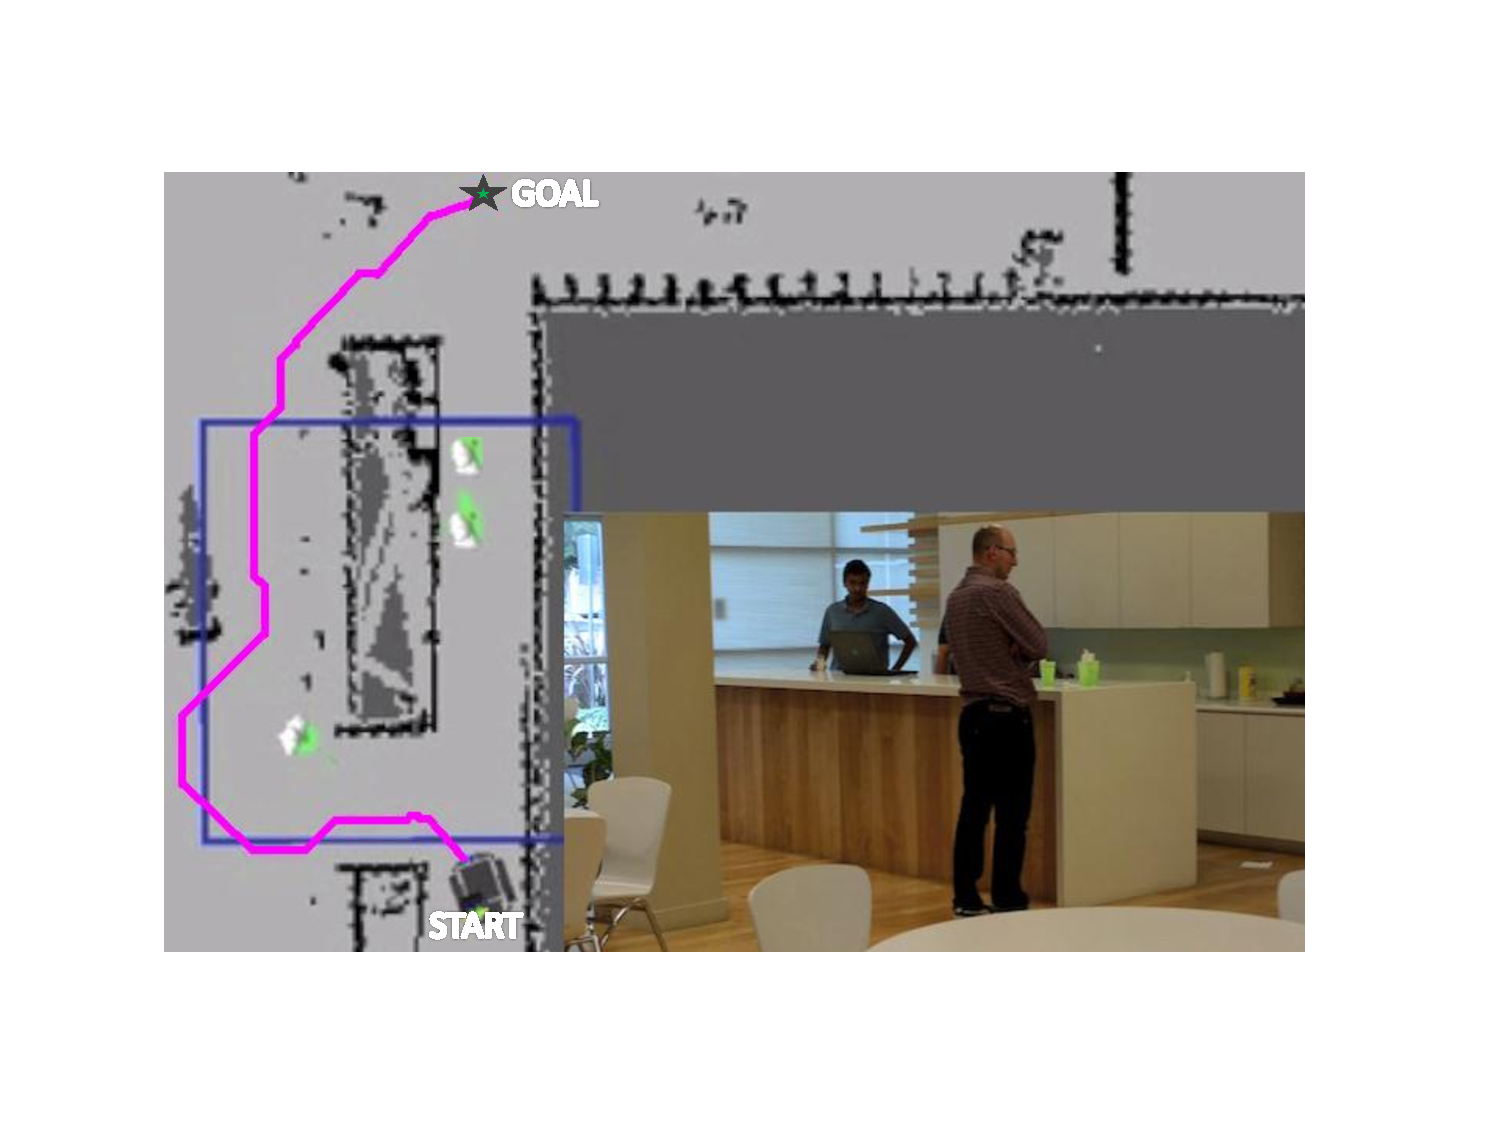
\includegraphics[width=0.6\columnwidth/2]{pics/kitchen5_crop}
        }%
        \subfigure[]{%
           \label{fig:corridor3}
           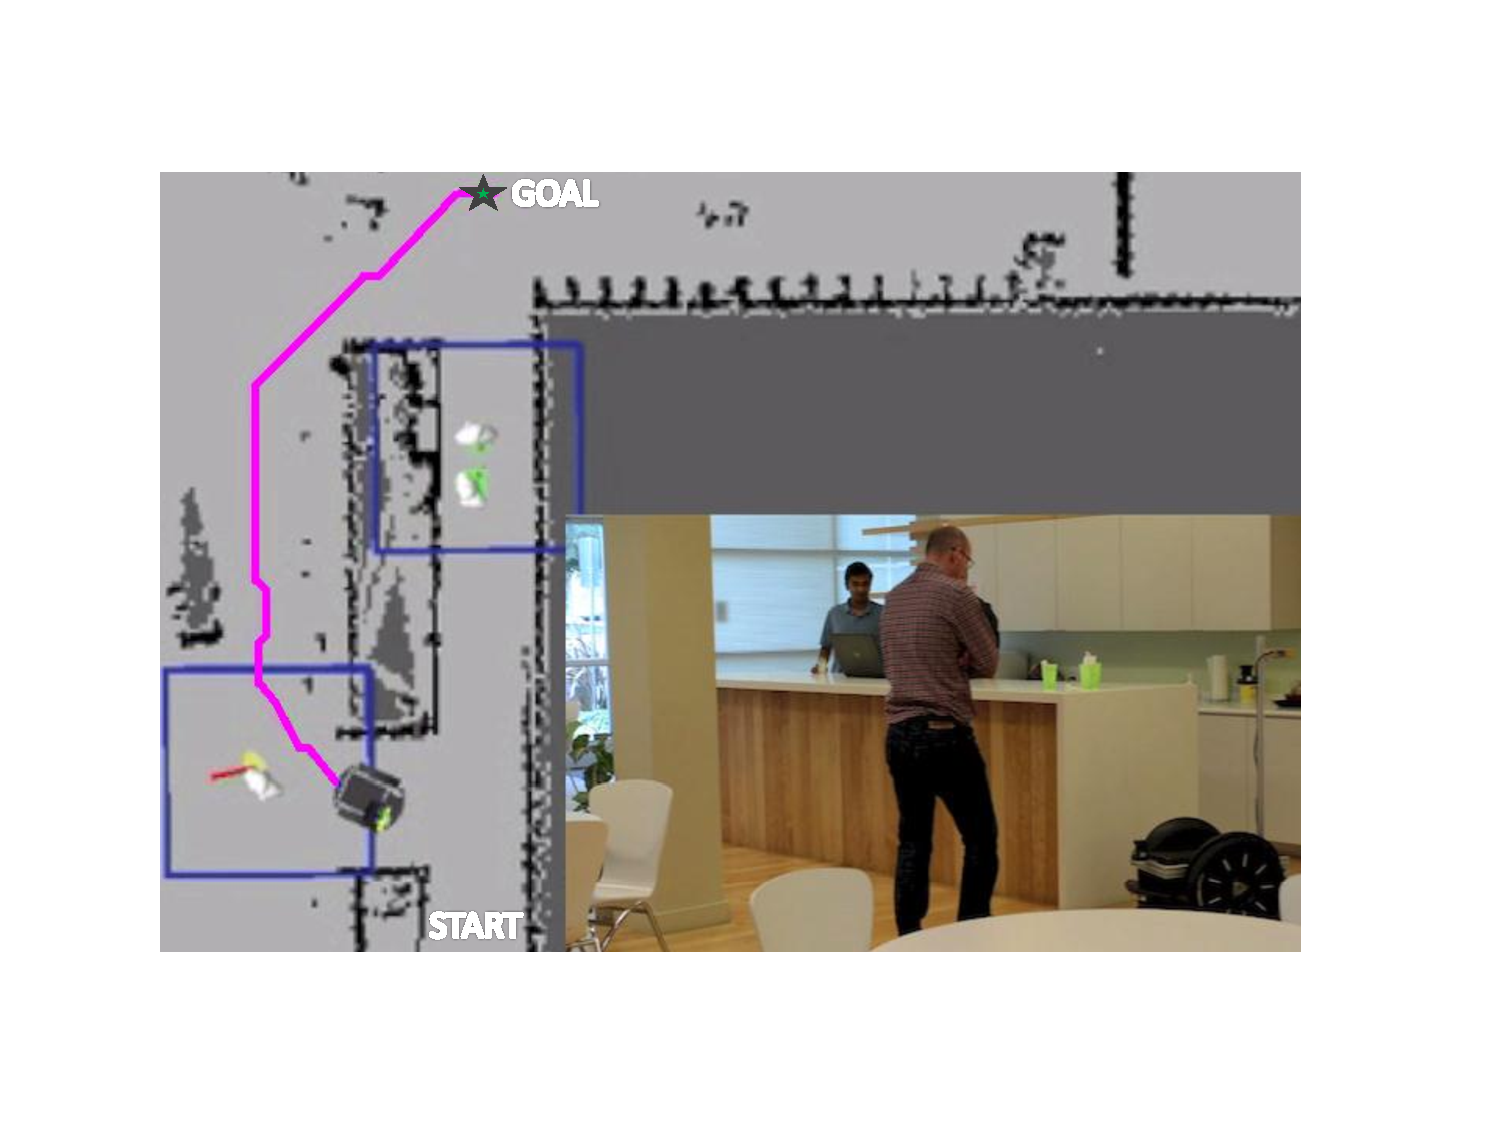
\includegraphics[width=0.6\columnwidth/2]{pics/kitchen6_crop}
        }
\subfigure[]{%
           \label{fig:corridor4}
           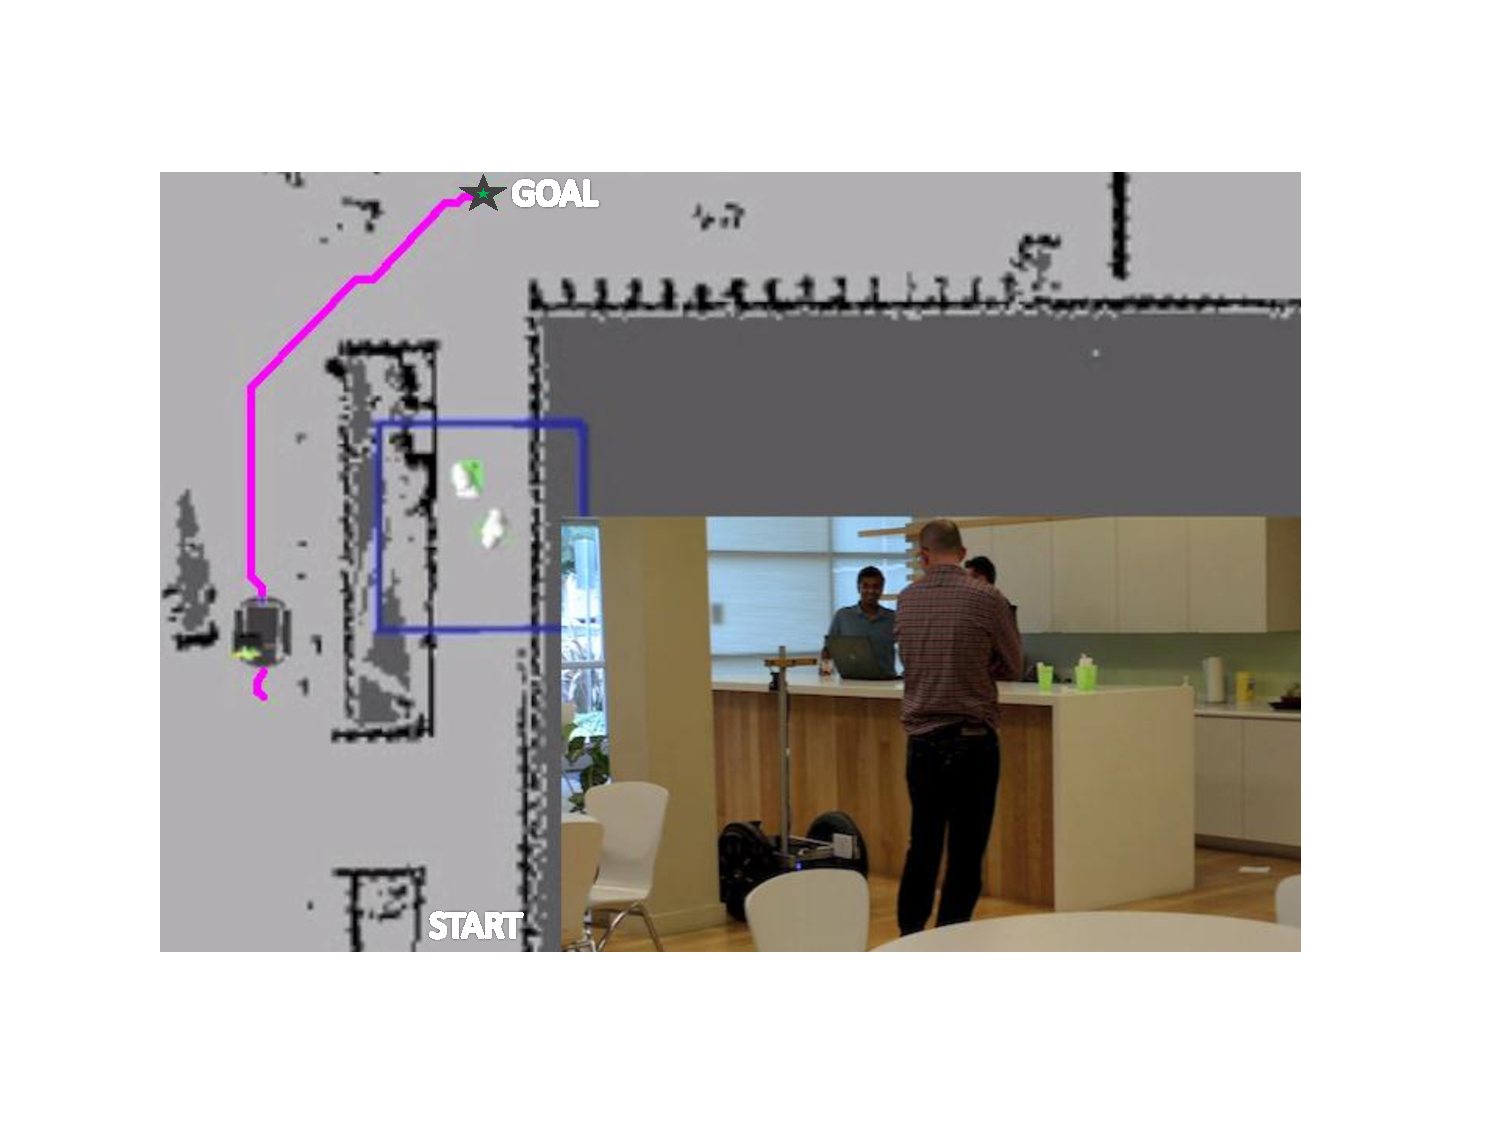
\includegraphics[width=0.6\columnwidth/2]{pics/kitchen7_crop}
        }
        
    \caption{%
	The Kitchen scenario. In the first run, there are two people blocking the path to the left and one person at the narrow corridor. a) robot decides to take the shorter route, because it would disturb one person instead of two. There is not enough space to pass, and dynamic planner assumes the person would get out of the bottleneck to give way. b) human behaves as robot anticipated and gets out of the narrow passage. robot slows down because it enters the human region. c) person gets back to his original position, robot reaches the goal. In the second run: d) there are two people at the narrow corridor and one person on the left. The robot decides to take the longer route and pass the third person from left. The safety cost from the two others would be too high if the robot took the direct route. e) the person steps back as he recognizes the robot. since the person has moved, the dynamic planner re-plans and decides to pass from right. f) after the robot passes the person, it proceeds to its goal.
     }%
   \label{fig:kitchen}
\end{figure}






\section{Speed Limits for Safe Navigation}
\label{sec:navigation_speed_limits}

In this chapter so far, we studied navigation planning that aims to generate human-friendly paths and safety of people must be at the utmost importance. In order to ensure the safety of people, we introduced \textbf{Safety Cost} in Section \ref{sec:navigation_global_planner} as well as repulsion forces in Section \ref{sec:navigation_path_refinement}. However, a seemingly safe path generated by our approach can still lead to an accident because it is may not be possible for the robot to track every human in the environment all the time. For example, when the robot is turning a corner, there is a risk that the robot suddenly encounters a person. Since the robot have finite deceleration, a collision may be unavoidable. The speeds that mobile robots should exhibit is also dependent on the context. For instance, a robot should move slowly and carefully in a hospital room. On the other hand, the robot may navigate faster in a long office corridor. The speed limits should better be provided by experts or the building owners, who govern how fast the robots should navigate in a particular environment.

In this section, we introduce speed maps that sets the speed limits for mobile robots in an environment. We claim that usage of such speed maps make the robots safer and potentially more efficient. The speed map designed for the second floor of the College of Computing building at Georgia Tech is shown in Figure \ref{fig:speed_map_irim}.

\begin{figure}[h!]
\centering
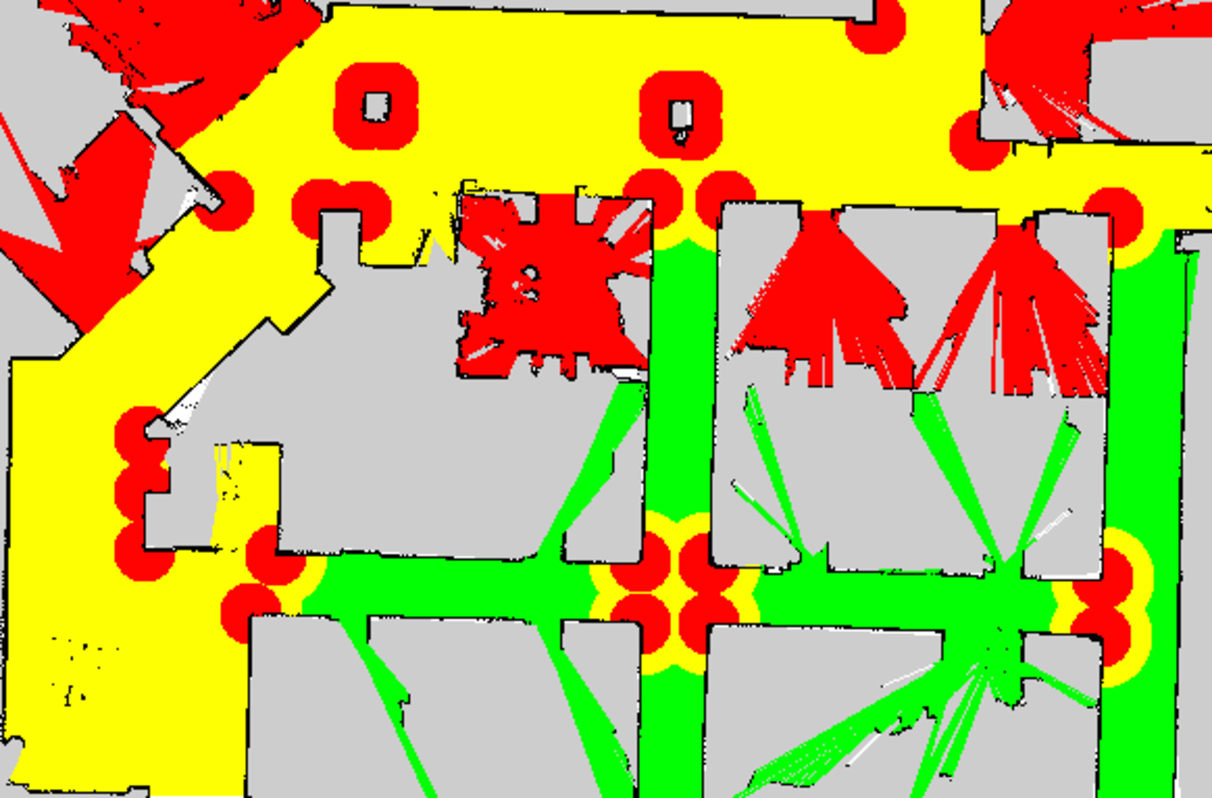
\includegraphics[width=0.6\textwidth]{pics/intro}
\caption{Designed speed limits for. The robot has to be relatively slow in red zones, can have moderate speed in yellow zones and is allowed to move relatively faster in green zones.}
\label{fig:speed_map_irim}
\end{figure}

The free spaces in this map are divided into three zones:
\begin{enumerate}
\item Green zone: The robot is allowed to travel at relatively faster speeds.
\item Yellow zone: Human interaction is possible, top speed is less than the maximum allowed
\item Red zone: Human encounter is probable, top speed is severely limited.
\end{enumerate}

This speed map is designed by hand using the following rules: Spaces corresponding to rooms and cubicles are covered as Red Zones. Blind corners are covered with a Red Zone close to corner and Yellow zone enclosing the Red Zone. Corridors are covered as Green Zones and the rest is covered as Yellow Zones. 

The speed map depicted in Figure \ref{fig:speed_map_irim} is designed by hand, however the speed map generation can be automatized using automatic room categorization and additional processing. Room segmentation has been proposed in an interactive fashion by \cite{diosi2005interactive}, as well as automatically, especially for creating topological maps \cite{mozos2007supervised}.

\subsection{Results}
\label{sec:navigation_speed_maps_results}

In this section, we evaluate the effect of applying speed limits in a navigation scenario. The robot is in an office environment and it has to turn a corner to reach the its goal. There is a person standing right around the corner and the person is not visible to the robot until it gets fairly close to the person. We had two conditions of speed limits:

\begin{itemize}
\item Condition 1: Fixed maximum linear speed of $v_{max}=1.0m/s$
\item Condition 2: Variable speed limits are used according to the speed map: $v_{max}(green)=1.5m/s$, $v_{max}(yellow)=0.5m/s$, $v_{max}(red)=0.15m/s$
\end{itemize}

In both conditions, standard ROS Navigation is used, which found the lowest cost path on a costmap consisting of costs from nearby obstacles. The robot detected the person using our multimodal person detection and tracking method described in Chapter \ref{chapter:multimodal_person_detection_and_tracking}. We analyze the distance/velocity of the robot as it encountered the human and measure the time to reach to the goal as evaluation metrics.

The section of the speed map including the corner is shown in Figure \ref{fig:nav_speed_map_corridor}. The trajectory with a fixed maximum speed is shown in Figure \ref{fig:nav_speed_map_black}. Note that the robot got dangerously close to the human while it turned the corner in Condition 1 and it was traveling with about $0.3m/s$ when it detected the person. The trajectory using the proposed speed limits is shown in Figure \ref{fig:nav_speed_map_color}. With this approach, the robot slowed down as it approached the corner, therefore allowing earlier detection of the human. The robot gave more space to the human in this case, the speed of the robot when it encountered the robot was  $0.15m/s$, half the speed of fixed max velocity case. Considering the speed of the robot and distance to the human at the time of encounter, we can say that the robot was safer.

The second metric we measured was the time to reach the goal. The robot was more efficient with the proposed approach, reaching the goal in $28s$ compared to $29.1s$.



\begin{figure}[ht!]
\centering
%
        \subfigure[]{%           
           \label{fig:nav_speed_map_corridor}
           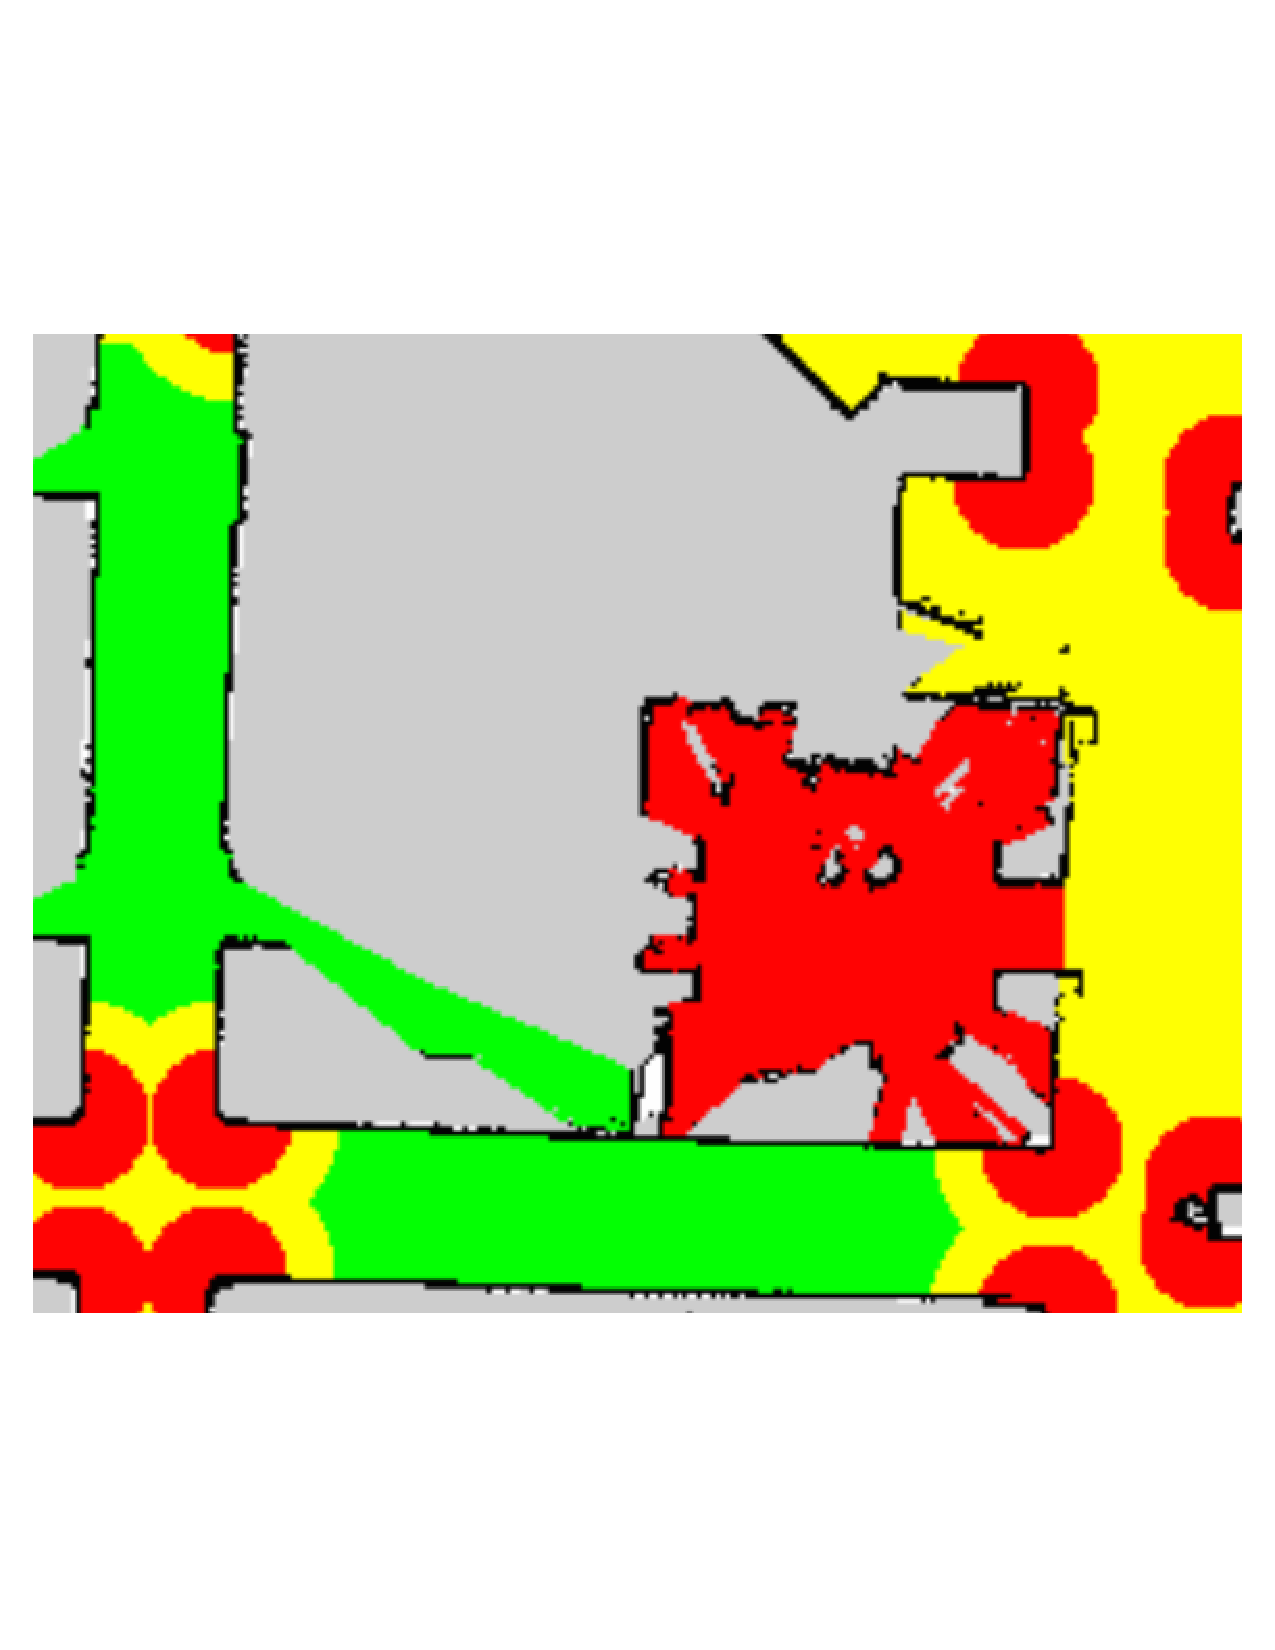
\includegraphics[width=0.5\textwidth]{pics/speed_map_corridor_pdf}
        } \\
        \subfigure[]{%
        	\label{fig:nav_speed_map_black}
            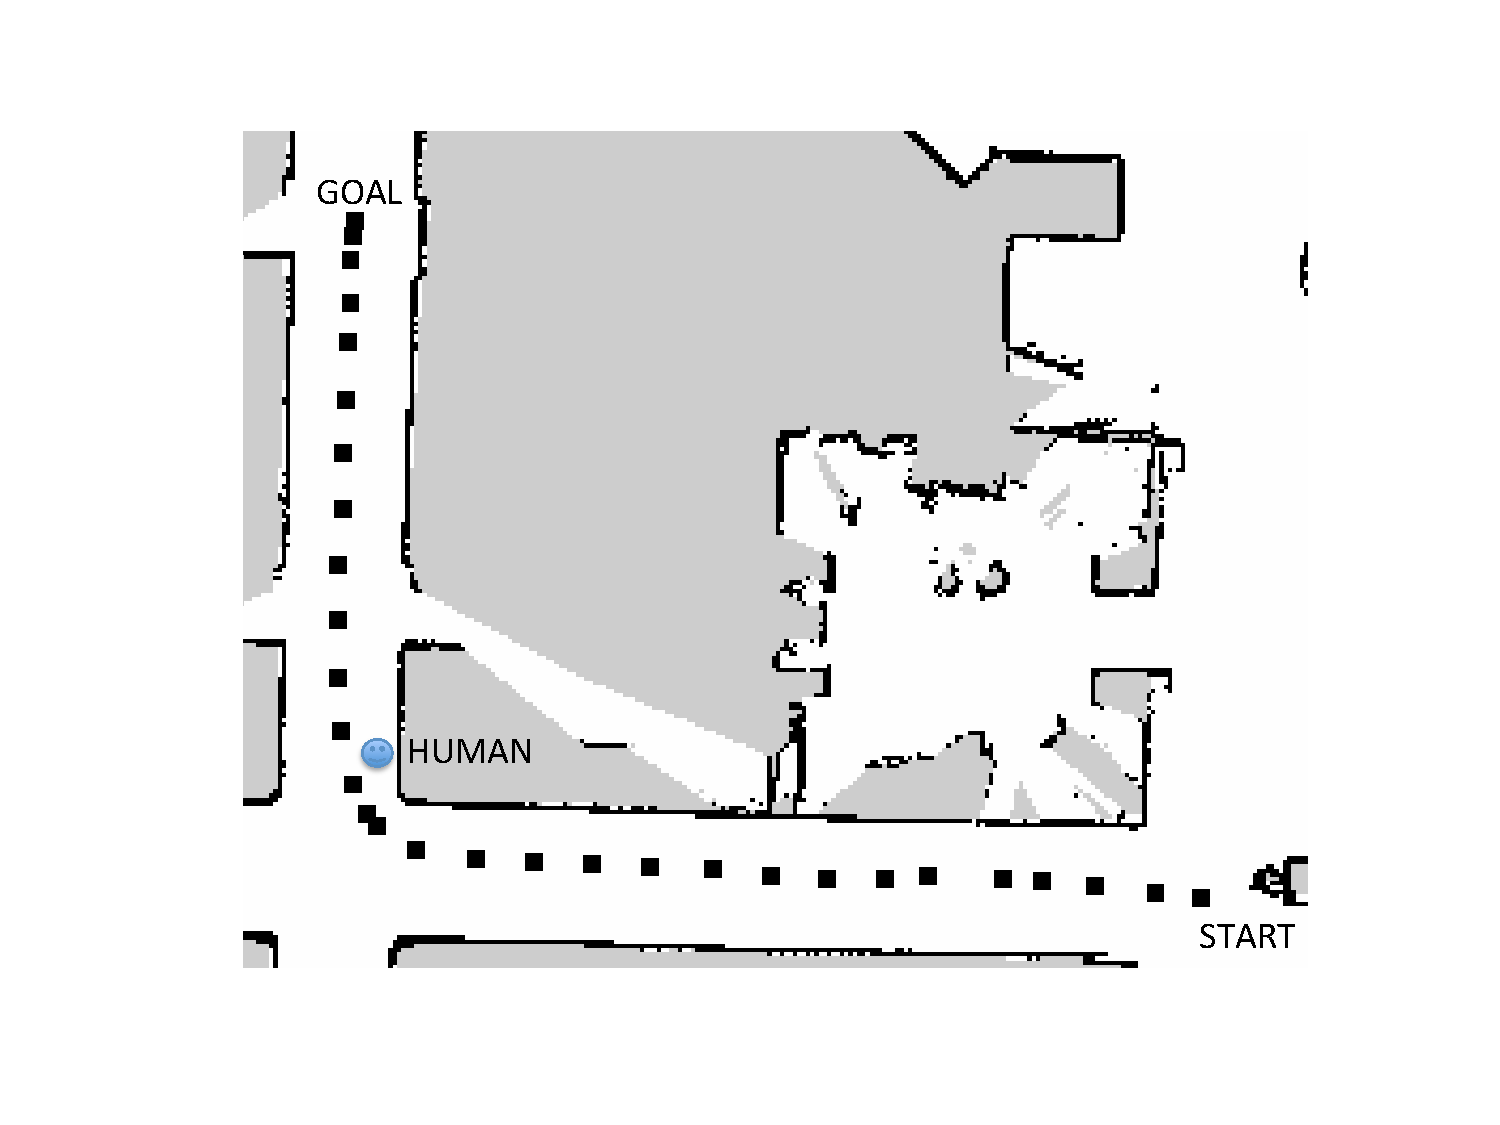
\includegraphics[width=0.5\textwidth]{pics/nav_noncolor_cropped}
        }%\\        
        \subfigure[]{%           
           \label{fig:nav_speed_map_color}
           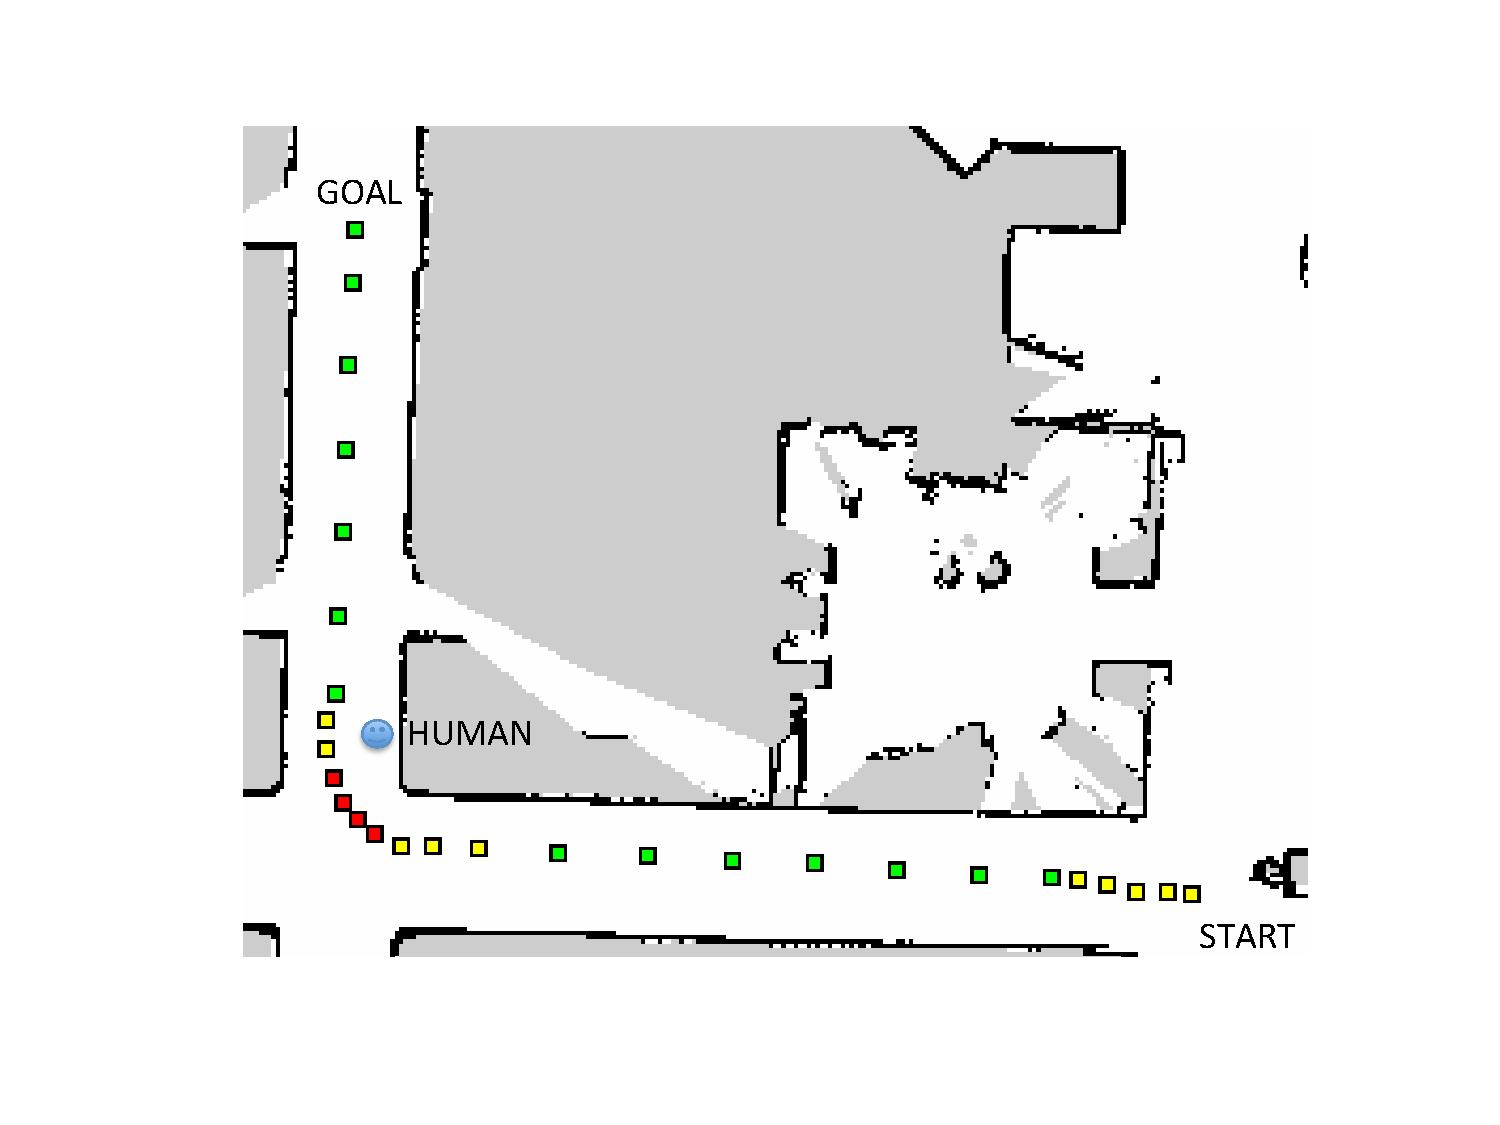
\includegraphics[width=0.5\textwidth]{pics/nav_colorr_cropped}
        }
    \caption{Comparison study of using a maximum top speed versus using location-dependent speed limits. Robot is given a fixed goal location. Right around the corner, there is a bystander human, who is not visible to the robot until the robot makes the turn. Points annotate robot position measured at fixed time intervals. a) Speed map of a corridor intersection at the second floor of College of Computing at Georgia Tech. b) Robot's top speed is fixed at $1.0m/s$. Note that the distance between robot positions are mostly constant. The robot gets very close to the bystander because it is moving relatively fast when it turned the corner. c) The robot is allowed to move with $1.5m/s$ in green, $0.5m/s$ in yellow and $0.15m/s$ in red zones. Colors of the sampled points on the path show the associated speed zone. It can be seen by looking at robot's positions that this approach was more gracious turning the corner and respecting human's personal space.}
   \label{fig:nav_speed_map_results}
\end{figure}

%%%%%%%%%%%%%%%%%%%%%%%%%%%%%%%%%%%%%%%%%%%%%%%%%%%%%%%%%%%%%%%%%%%%%%